% ----------------------------------------------------
% Magic Comments for LaTeX-editors (TeXstudio, VSCode with LaTeX Workshop extension...)
% !TeX encoding = utf8
% !TeX spellcheck = de_DE
% !TeX program = pdflatex
% !BIB program = biber
% ----------------------------------------------------

% ----------------------------------------------------
% Load the HfTL-Thesis class
\documentclass[
% Select the main Language of your thesis here. Titlepage, captions and statement of authorship will change accordingly:
%
% ngerman% - Deutsch (default)
% USenglish % - American english
% UKenglish % - British english
% numeric   % (default) use numeric citation style sorted by the occurence in text: [5]
% alphabetic % - use alphabetic citation style: [Lau95]
% authoryear % - use authoryear citation style: Laubach 1995
]{hftlthesis}
% ----------------------------------------------------

% ----------------------------------------------------
% Set your custom options here. See https://komascript.de/~mkohm/scrguide.pdf for possibilities.

%\KOMAoption{twoside}{true} % Enable double sided layout
%\KOMAoption{BCOR}{8.25mm} % Binding Correction, adds the specified margin to the inner side of the page (left on single sided layout). This is to compensate lost page margin due to binding.

% ----------------------------------------------------

% ----------------------------------------------------
% Load your own packages here
\usepackage{blindtext} % Only for demonstration purposes. Can be removed!
\usepackage{todonotes}
\usepackage{float}
\usepackage{tikz, pgfplots} % To create diagrams and figures directly with LaTeX
\usepackage{listings} % support for Sourcecodelistings. For more advanced, prettier highlighting use the minted package instead (https://github.com/gpoore/minted) -> Requires Python with Pygments installed.
\usepackage{siunitx} % provides support for SI unit handling
\usepackage[useregional]{datetime2} % support for formatted date
\usepackage{booktabs}
\usepackage{amssymb}
\usepackage{longtable}

% ----------------------------------------------------

% ----------------------------------------------------
% Variables for Titlepage, PDF properties...
% Below are the default values. Comment them out to change them!

%\university{Hochschule für Telekommunikation Leipzig (FH)}
%\institute{Institut für Telekommunikationsinformatik}
%\documentKind{Abschlussarbeit zur Erlangung des akademischen Grades}
%\forDegree{Bachelor of Engineering}
%
\topic{\enquote{Untersuchung des Stromverbrauchs von verschiedenen Algorithmen und deren Implementierung auf mobilen Geräten}}
%
\thesisAuthor{Niklas Kluge}
\authorDateOfBirth{27.06.1996}
\authorPlaceOfBirth{Wernigerode}
%
\handInDate{\DTMdate{2020-10-31}} %formatted custom date
%
\firstReviewerName{Prof. Dr. Ulf Schemmert}
\firstReviewerInstitution{Hochschule für Telekommunikation Leipzig}
\firstReviewerInstitutionStreet{Gustav-Freytag-Straße 43-45}
\firstReviewerInstitutionPlace{04277 Leipzig}
%
\secondReviewerName{Philipp Dockhorn, M. Eng.}
\secondReviewerInstitution{Hochschule für Telekommunikation Leipzig}
\secondReviewerInstitutionStreet{Gustav-Freytag-Straße 43-45}
\secondReviewerInstitutionPlace{04277 Leipzig}

% ----------------------------------------------------

% ----------------------------------------------------
% Include own references
\addbibresource{References/online.bib}
\addbibresource{References/3gpp.bib}
\addbibresource{References/etsi.bib}
\addbibresource{References/itut.bib}
%\addbibresource{References/rfc.bib}
\addbibresource{References/niklasLiteratur.bib}
% ----------------------------------------------------
% ----------------------------------------------------
% Set a list of directories, where graphics are stored, so you dont have to prepend the subdirectory in \includegraphics. The "Graphics" folder is set by default.

%\graphicspath{{./Graphics/}, {./Images}}
% ----------------------------------------------------

% ----------------------------------------------------
% Load acronym definitions
\newacronym{3gpp}{3GPP}{Third Generation Partnership Project}
\newacronym{aaa}{AAA}{Authentication, Authorisation and Accounting}
\newacronym{aac-eld}{AAC-ELD}{Advanced Audio Coding-Enhanced Low Delay}
\newacronym{acr}{ACR}{Absolute Category Rating}
\newacronym{af}{AF}{Application Function}
\newacronym{agcf}{AGCF}{Access Gateway Control Function}
\newacronym{agch}{AGCH}{Access Grant Channel}
\newacronym{ajax}{AJAX}{Asynchronous JavaScript and XML}
\newacronym{amr}{AMR}{Adaptive Multi Rate}
\newacronym{amr-wb}{AMR-WB}{Adaptive Multirate-Wideband}
\newacronym{ape}{APE}{AJAX Push Engine}
\newacronym{api}{API}{Application Programming Interface}
\newacronym{apn}{APN}{Access Point Name}
\newacronym{appserv}{AS}{Application Server}
\newacronym{armgw}{A/R-MGW}{Access/Residential-Media Gateway}
\newacronym{arvgw}{A/R-VGW}{Access/Residential-Voice over IP-Gateway}
\newacronym{as}{AS}{Access Stratum}
\newacronym{auc}{AuC}{Authentication Centre}
\newacronym{avp}{AVP}{Attribute-Value-Pairs}
\newacronym{bcch}{BCCH}{Broadcast Control Channel}
\newacronym{bgcf}{BGCF}{Breakout Gateway Control Function}
\newacronym{bsc}{BSC}{Base Station Controller}
\newacronym{bts}{BTS}{Base Transceiver Station}
\newacronym{ca}{CA}{Certificate Authority}
\newacronym{ca_mac}{CA}{Collision Avoidance}
\newacronym{camel}{CAMEL}{Customised Application for Mobile network Enhanced Logic}
\newacronym{cc}{CC}{Call Control, Country Code}
\newacronym{celp}{CELP}{Code-Excited Linear-Prediction}
\newacronym{celt}{CELT}{Constrained Energy Lapped Transform}
\newacronym{cli}{CLI}{Command Line Interface}
\newacronym{cm}{CM}{Connection Management}
\newacronym{cng}{CNG}{Comfort Noise Generation}
\newacronym{cod}{CoD}{Content on Demand}
\newacronym{cp}{CP}{Control Plane}
\newacronym{cpe}{CPE}{Customer-Premises Equipment}
\newacronym{cs}{CS}{Circuit Switched}
\newacronym{cs-acelp}{CS-ACELP}{Conjugate-Structure Algebraic-Code Excited Linear-Prediction}
\newacronym{cscf}{CSCF}{Call/Session Control Function}
\newacronym{csfb}{CSFB}{Circuit Switched Fallback}
\newacronym{csma}{CSMA}{Carrier Sense Medium Access}
\newacronym{css}{CSS}{Cascading Style Sheets}
\newacronym{db}{DB}{Database}
\newacronym{dom}{DOM}{Document Object Model}
\newacronym{dscp}{DSCP}{Differentiated Services Code Points}
\newacronym{dtls}{DTLS}{Datagram Transport Layer Security}
\newacronym{dtx}{DTX}{Discontinuous Transmission}
\newacronym{dv}{DV}{Delay Variation}
\newacronym{e-rab}{E-RAB}{E-UTRAN Radio Access Bearer}
\newacronym{e-utran}{E-UTRAN}{Evolved UMTS Radio Access Network}
\newacronym{e2e}{E2E}{End-to-End}
\newacronym{edge}{EDGE}{Enhanced Data rates for GSM Evolution}
\newacronym{edss1}{EDSS1}{European Digital Subscriber System No. 1}
\newacronym{eir}{EIR}{Equipment Identity Centre, Equipment Identity Register}
\newacronym{epc}{EPC}{Evolved Packet Core}
\newacronym{epg}{EPG}{Electronic Program Guide}
\newacronym{eps}{EPS}{Evolved Packet System}
\newacronym{etsi}{ETSI}{European Telecommunication Standards Institute}
\newacronym{etsi-tispan}{ETSI-TISPAN}{ETSI-Telecommunications and Internet converged Services and Protocols for AdvancedNetworking}
\newacronym{facch}{FACCH}{Fast Associated Control CHannel}
\newacronym{fb}{FB}{Fullband}
\newacronym{fcch}{FCCH}{Frequency Correction CHannel}
\newacronym{fec}{FEC}{Forward Error Correction}
\newacronym{fmc}{FMC}{Fixed Mobile Convergence}
\newacronym{fokus}{FOKUS}{Fraunhofer-Institut für Offene Kommunikationssysteme}
\newacronym{fr}{FR}{Full Rate}
\newacronym{geran}{GERAN}{GSM EDGE Radio Access Network}
\newacronym{ggsn}{GGSN}{Gateway GPRS Support Node}
\newacronym{gmm}{GMM}{GPRS Mobility Management}
\newacronym{gmsc}{GMSC}{Gateway MSC}
\newacronym{gprs}{GPRS}{General Packet Radio Service}
\newacronym{gsm}{GSM}{Global System for Mobile communications}
\newacronym{gsma}{GSMA}{GSM Association}
\newacronym{gtp}{GTP}{GPRS Tunneling Protocol}
\newacronym{gui}{GUI}{Graphical User Interface}
\newacronym{gw}{GW}{Gateway}
\newacronym{hd}{HD}{High Definition}
\newacronym{hlr}{HLR}{Home Location Register}
\newacronym{hr}{HR}{Half Rate}
\newacronym{hscsd}{HSCSD}{High-Speed Circuit-Switched Data}
\newacronym{hss}{HSS}{Home Subscriber Server}
\newacronym{html5}{HTML5}{Hypertext Markup Language Version 5}
\newacronym{http}{HTTP}{Hypertext Transfer Protocol}
\newacronym{iad}{IAD}{Integrated Access Device}
\newacronym{iana}{IANA}{Internet Assigned Numbers Authority}
\newacronym{ibcf}{IBCF}{Interconnection Border Control Function}
\newacronym{ibgf}{IBGF}{Interconnection Border Gateway Function}
\newacronym{ice}{ICE}{Interactive Connectivity Establishment}
\newacronym{i-cscf}{I-CSCF}{Interrogating-CSCF}
\newacronym{iesg}{IESG}{Internet Engineering Steering Group}
\newacronym{ietf}{IETF}{Internet Engineering Task Force}
\newacronym{imei}{IMEI}{International Mobile Equipment Identity}
\newacronym{ims}{IMS}{IP Multimedia Subsystem}
\newacronym{imscm}{IMSCM}{IMS-Client-Manager}
\newacronym{imsi}{IMSI}{International Mobile Subscriber Identity}
\newacronym{imssf}{IM-SSF}{IP Multimedia Service Switching Function}
\newacronym{imt}{IMT}{International Mobile Telecomunication}
\newacronym{inap}{INAP}{Intelligent Network Application Part}
\newacronym{ip}{IP}{Internet Protocol}
\newacronym{ip-can}{IP-CAN}{Internet Protocol- Connectivity Access Network}
\newacronym{ipdv}{IPDV}{IP Delay Variation}
\newacronym{iper}{IPER}{IP Packet Error Ratio}
\newacronym{iplr}{IPLR}{IP Packet Loss Ratio}
\newacronym{iptd}{IPTD}{IP Transfer Delay}
\newacronym{iptv}{IPTV}{Internet Protocol Television}
\newacronym{isc}{ISC}{IMS Service Control}
\newacronym{isdn}{ISDN}{Integrated Services Digital Network}
\newacronym{iso/osi}{ISO/OSI}{Open System Interconnection/International Organization for Standardization}
\newacronym{isup}{ISUP}{ISDN User Part}
\newacronym{itu}{ITU}{International Telecommunication Union}
\newacronym{itu-t}{ITU-T}{International Telecommunications Union-Telecommunication Standardization Sector}
\newacronym{json}{JSON}{JavaScript Object Notation}
\newacronym{la}{LA}{Location Area}
\newacronym{label}{API}{Application Programming Interface}
\newacronym{lcp}{LCP}{Link Control Protocol}
\newacronym{llc}{LLC}{Logical Link Control}
\newacronym{lp}{LP}{Linear Prediction}
\newacronym{lte}{LTE}{Long Term Evolution}
\newacronym{m2m}{M2M}{Machine to Machine Communication}
\newacronym{mac}{MAC}{Medium Access Control}
\newacronym{mac_encryption}{MAC}{Message Authentication Code (encryption context)}
\newacronym{map}{MAP}{Mobile Application Part}
\newacronym{mcf}{MCF}{Media Control Function}
\newacronym{mdct}{MDCT}{Modified Discrete Cosine Transform}
\newacronym{mdf}{MDF}{Media Delivery Function}
\newacronym{mfv}{MFV}{Mehrfach Frequenz Wahlverfahren/Tonwahl}
\newacronym{mgc}{MGC}{Media Gateway Controler}
\newacronym{mgcf}{MGCF}{Media Gateway Control Function}
\newacronym{mgw}{MGW}{Media Gateway Function}
\newacronym{mime}{MIME}{Multipurpose Internet Mail Extensions}
\newacronym{mm}{MM}{Mobility Management}
\newacronym{mme}{MME}{Mobile Management Entity}
\newacronym{mos}{MOS}{Mean Opinion Score}
\newacronym{mrf}{MRF}{Multimedia Resource Function}
\newacronym{mrfc}{MRFC}{Multimedia Resource Function Controller}
\newacronym{mrfp}{MRFP}{Multimedia Resource Function Processor}
\newacronym{msc}{MSC}{Mobile Switching Centre}
\newacronym{msisdn}{MSISDN}{Mobile Subscriber ISDN Number}
\newacronym{n-pvr}{N-PVR}{Network-Personal Video Recorder}
\newacronym{napt}{NAPT}{Network Address and Port Translation}
\newacronym{nas}{NAS}{Non-Access Stratum}
\newacronym{nas_server}{NAS}{Network Access Server}
\newacronym{nass}{NASS}{Network Attachment Subsystem}
\newacronym{nat}{NAT}{Network Address Translation}
\newacronym{nb}{NB}{Narrowband}
\newacronym{nfv}{NFV}{Network Function Virtualization}
\newacronym{ngn}{NGN}{Next Generation Network}
\newacronym{nni}{NNI}{Network-Network Interface}
\newacronym{nodeb}{NodeB}{Funkbasisstation im UTRAN}
\newacronym{nsapi}{NSAPI}{Network Service Access Point Identifier}
\newacronym{ntba}{NTBA}{Network Termination for ISDN Basic rate Access / Netzterminator Basisanschluss}
\newacronym{osa}{OSA}{Open Service Access}
\newacronym{osascs}{OSA-SCS}{Open Service Access - Service Capability Server}
\newacronym{osgi}{OSGi}{Open Services Gateway initiative}
\newacronym{osi}{OSI}{Open System Interconnection}
\newacronym{ott}{OTT}{Over The Top Anwendungen}
\newacronym{p-cscf}{P-CSCF}{Proxy Call Session Control Function}
\newacronym{pcc}{PCC}{Policy and Charging Control}
\newacronym{pcef}{PCEF}{Policy Control Enforcement Function}
\newacronym{pch}{PCH}{Paging Channel}
\newacronym{pcrf}{PCRF}{Policy and Charging Rules Function}
\newacronym{pcu}{PCU}{Packet Control Unit}
\newacronym{pdn}{PDN}{Public Data Network, Packet Data Network}
\newacronym{pdn-gw}{PDN-GW}{Packet Data Network Gateway}
\newacronym{pelr}{PELR}{Packet Error Loss Rate}
\newacronym{pes}{PES}{PSTN/ISDN Emulation Subsystem}
\newacronym{pesq}{PESQ}{Perceptual Evaluation of Speech Quality}
\newacronym{pgw}{PGW}{Packet Data Network Gateway}
\newacronym{php}{PHP}{PHP: Hypertext Preprocessor}
\newacronym{plmn}{PLMN}{Public Land Mobile Network}
\newacronym{plr}{PLR}{Packet Loss Rate}
\newacronym{pnai}{PNAI}{Personal Network Administration Interface}
\newacronym{polqa}{POLQA}{Perceptual Objective Listening Quality Assessment}
\newacronym{pots}{POTS}{Plain Old Telephone System}
\newacronym{ppv}{PPV}{Pay-Per-View}
\newacronym{ps}{PS}{Packet Switched, Location Probability}
\newacronym{pss}{PSS}{PSTN/ISDN Simulation Subsystem}
\newacronym{pstn}{PSTN}{Public Switched Telephone Network}
\newacronym{qci}{QCI}{QoS Class Identifier}
\newacronym{qoe}{QoE}{Quality of Experience}
\newacronym{qos}{QoS}{Quality of Service}
\newacronym{ra}{RA}{Routing Area, Random mode request information field}
\newacronym{rab}{RAB}{Radio Access Bearer, Access Burst}
\newacronym{rat}{RAT}{Radio Access Technology}
\newacronym{rach}{RACH}{Random Access Channel}
\newacronym{racs}{RACS}{Resource Admission Control Subsystem}
\newacronym{radius}{RADIUS}{Remote Authentication Dial In User Service}
\newacronym{rcs}{RCS}{Rich Communication Suite}
\newacronym{rlc}{RLC}{Radio Link Control}
\newacronym{rnc}{RNC}{Radio Network Controller}
\newacronym{rpe-ltp}{RPE-LTP}{Regular Pulse Excitation - Long Term Prediction}
\newacronym{rr}{RR}{Radio Resources}
\newacronym{rrc}{RRC}{Radio Resource Control}
\newacronym{rtc}{RTC}{Real Time Communication}
\newacronym{rtcp}{RTCP}{RTP Control Protocol}
\newacronym{rtp}{RTP}{Realtime Transport Protocol}
\newacronym{rtsp}{RTSP}{Real-Time Streaming Protocol}
\newacronym{rtt}{RTT}{Round Trip Time}
\newacronym{sacch}{SACCH}{Slow Associated Control Channel}
\newacronym{sai}{SAI}{Service Attachment Information}
\newacronym{sapi}{SAPI}{Service Access Point Identifier}
\newacronym{scf}{SCF}{Service Control Function}
\newacronym{sch}{SCH}{Synchronisation Channel}
\newacronym{s-cscf}{S-CSCF}{Serving-CSCF}
\newacronym{sctp}{SCTP}{Stream Control Transmission Protocol}
\newacronym{sd}{SD}{Standard Definition}
\newacronym{sdcch}{SDCCH}{Stand-Alone Dedicated Control Channel}
\newacronym{sdf}{SDF}{Service Discovery Function}
\newacronym{sdma}{SDMA}{Space Division Multiple Access}
\newacronym{sdp}{SDP}{Session Description Protocol}
\newacronym{servgw}{ServGW}{Serving Gateway}
\newacronym{sgsn}{SGSN}{Serving GPRS Support Node}
\newacronym{sgw}{S-GW}{Signaling Gateway}
\newacronym{sigtran}{SIGTRAN}{ZGSNr.7 Signaling Transport Protocol Suite}
\newacronym{silk}{SILK}{SILK Speech codec}
\newacronym{sip}{SIP}{Session Initiation Protocol}
\newacronym{sipas}{SIP AS}{SIP Application Server}
\newacronym{slf}{SLF}{Subscriber Location Function}
\newacronym{sms}{SMS}{Short Message Service}
\newacronym{srtp}{SRTP}{Secure Real-Time Transport Protocol}
\newacronym{ss}{SS}{Supplementary Service}
\newacronym{sscon}{SSCON}{Session Controller}
\newacronym{ssf}{SSF}{Service Selection Function}
\newacronym{ssi}{SSI}{Service Selection Information}
\newacronym{ssrc}{SSRC}{Synchronization Source}
\newacronym{stun}{STUN}{Session Traversal Utilities for NAT}
\newacronym{swb}{SWB}{Super-Wideband}
\newacronym{tch}{TCH}{Traffic Channel}
\newacronym{tcp}{TCP}{Transmission Control Protocol}
\newacronym{td}{TD}{Transfer Delay}
\newacronym{tdd}{TDD}{Time Division Duplex}
\newacronym{tispan}{TISPAN}{Telecommunications and Internet converged Services and Protocols for Advanced Networking}
\newacronym{tmsi}{TMSI}{Temporary Mobile Subscriber Identity}
\newacronym{tn}{TN}{Termination Node, Timeslot Number}
\newacronym{toc}{TOC}{Table-Of-Contents}
\newacronym{turn}{TURN}{Traversal Using Relays around NAT}
\newacronym{tv}{TV}{Television}
\newacronym{ua}{UA}{User Agent}
\newacronym{udp}{UDP}{User Datagram Protocol}
\newacronym{ue}{UE}{User Equipment}
\newacronym{umts}{UMTS}{Universal Mobile Telecommunications System}
\newacronym{uni}{UNI}{User-Network Interface}
\newacronym{up}{UP}{User Plane}
\newacronym{upsf}{UPSF}{User Profile Server Function}
\newacronym{uri}{URI}{Uniform Resource Identifier}
\newacronym{url}{URL}{Uniform Resource Locator}
\newacronym{utran}{UTRAN}{Universal Terrestrial Radio Access Network}
\newacronym{vad}{VAD}{Voice Activity Dedection}
\newacronym{vbr}{VBR}{Variable Bit  Rate}
\newacronym{vgw}{VGW}{Voice over IP-Gateway}
\newacronym{vlc}{VLC}{VideoLan Client}
\newacronym{vod}{VoD}{Video on Demand}
\newacronym{voip}{VoIP}{Voice Over IP}
\newacronym{volga}{VoLGA}{Voice over LTE via Generic Access}
\newacronym{volte}{VoLTE}{Voice over LTE}
\newacronym{w3c}{W3C}{World Wide Web Consortium}
\newacronym{waf}{WAF}{WebRTC Authentication Function}
\newacronym{wb}{WB}{Wideband}
\newacronym{webrtc}{WebRTC}{Web Real-Time Communication}
\newacronym{wlan}{WLAN}{Wireless Local Area Network}
\newacronym{wqsf}{WQSF}{WebRTC QoS Signalling Function}
\newacronym{wwsf}{WWSF}{WebRTC Web Server Function}
\newacronym{xdsl}{xDSL}{any Digital Subscriber Line}
\newacronym{xml}{XML}{Extended MarkupLanguage}
\newacronym{zgs nr.7}{ZGS Nr.7}{Zentrales Zeichengabesystem Nr.7}
\newacronym{sdk}{SDK}{Software Developoment Kit}
\newacronym{ui}{UI}{User Interface}
\newacronym{kb}{KB}{Kilo Byte}
\newacronym{mio}{Mio}{Millionen}
\newacronym{gb}{GB}{Giga Byte}
\newacronym{mAh}{mAh}{Milliamperestunden}
\newacronym{ppi}{ppi}{Pixel per Inch}
\newacronym{cpu}{CPU}{Central Processing Unit}
\newacronym{soc}{SoC}{System on a Chip}
\newacronym{ghz}{GHz}{Gigahertz}
\newacronym{html}{HTML}{Hypertext Markup Language}
\newacronym{adb}{ADB}{Android-Debug-Bridge}
\newacronym{ascii}{ASCII}{American Standard Code for Information Interchange}
\newacronym{wifi}{Wfi}{Wireless Local Area Network}
\newacronym{mV}{mV}{Millivolt}
\newacronym{mA}{mA}{Milliampere}
\newacronym{jvm}{JVM}{Java Virtual Machine}
\newacronym{smtp}{SMTP}{Simple Mail Transfer Protocol}
\newacronym{utf-8}{UTF-8}{8-Bit UCS Transformation Format}
\newacronym{rfc}{RFC}{Request for Comments }
\newacronym{oom}{OOM}{Out of Memory}
\newacronym{ms}{ms}{Millisekunden}
\newacronym{w}{W}{Watt}
\makenoidxglossaries % index acronyms

% ----------------------------------------------------

% ----------------------------------------------------
% The document body. Start your work here.
\begin{document}
\frontmatter % page numbers as small roman letters
\maketitle % print the titlepage
\cleardoublepage % start a new page

\chapter{Vorwort}
An dieser Stelle möchte ich mich bei Herrn Dr. Schemmert für die zuverlässige Betreuung bedanken. Mit seinen Ratschlägen half  Herr Schemmert mir bei der Findung zahlreicher Denkansätze, welche in der vorliegenden Arbeit Einzug erhalten haben. Des Weiteren möchte ich meiner Familie danken, die mir trotz familiärer Schicksalsschläge und gesundheitlicher Probleme während des Bearbeitungszeitraums genug Kraft geben konnte, um diese Arbeit rechtzeitig fertigzustellen. % include the file Content/vorwort.tex
\cleardoublepage

\tableofcontents %print the table of contents
\cleardoublepage

\printnoidxglossary[type=\acronymtype] % print the list of abbreviations
\cleardoublepage

\listoffigures % print the list of figures
\cleardoublepage

\listoftables % print the list of tables
\cleardoublepage

\lstlistoflistings % print the list of source codes
\cleardoublepage	
	
\mainmatter %page numbers arabic, beginning from 1	

%Include the example document
%% !TeX root = ../my-thesis.tex
\chapter{Beispiel zur Nutzung}
\section{Abkürzungen und Zitate}
Jedes Acronym hat einen Identifier, der komplett klein geschrieben wird. Im Beispiel: volte~-~nicht zu verwechseln mit der Abkürzung selbst (hier VoLTE). Im Abkürzungsverzeichnis werden alle Abkürzungen aufgelistet, mit allen Stellen, an denen sie Dokument verwendet wurden. 

\begin{minipage}{.6\textwidth}
\begin{lstlisting}[language=latex]
\ac{volte} % Erste Verwendung: 
% Langform (Abkürzung)
\ac{volte} % Zweite Verwendung: Abkürzung
\acs{isdn} % s = short: Abkürzung
\acl{ims} % l = long: Langform
\acf{iad} % f = full: Langform (Kurzform)
\end{lstlisting}   
\end{minipage}
\begin{minipage}{.4\textwidth}
	\footnotesize
	\textbf{Ergibt:}\\
	\ac{volte}\\
	\ac{volte}\\
	\acs{isdn}\\
	\acl{ims}\\
	\acf{iad} 
\end{minipage}

Bei der ersten Verwendung, wird die Langform ausgegeben, alle weitere Nutzungen der Abkürzung ergeben nur die Kurzform. Somit muss man nicht überlegen, ob die Abkürzung schon mal verwendet wurde, wie folgender Satz zeigt: 

\Ac{volte} ist eine tolle Erfindung \cite{3GPP.TS.24.228.v5.15.0}. Die Signalisierung läuft über das \ac{sip}~\cite{wikiNik}. \cite[S.~23]{fernandezgallardo_InstitutFurSoftwaretechnik_2017}
\cite[S.~50]{arnold2000java}

Auch das Zitieren von Quellen ist mit \LaTeX{} ein Kinderspiel! Treffe ich eine Aussage, so muss ich sie belegen~\cite{rfc2693}. Dies geschieht mit dem Befehl \lstinline[language=latex]|\cite{<bibid>}|. Mehrere Quellen werden durch eine kommagetrennte Liste an \texttt{BibIDs} im \texttt{cite} Befehl zitiert: \lstinline[language=latex]|\cite{<bibid1>, <bibid2>, <bibid2>}| ergibt: schrägstrich cite{rfc1, rfc1754, rfc1971}. Alle zitierten Quellen landen im Literaturverzeichnis.
\section{Bilder und Verweise}
\begin{figure}[ht]
	\centering
	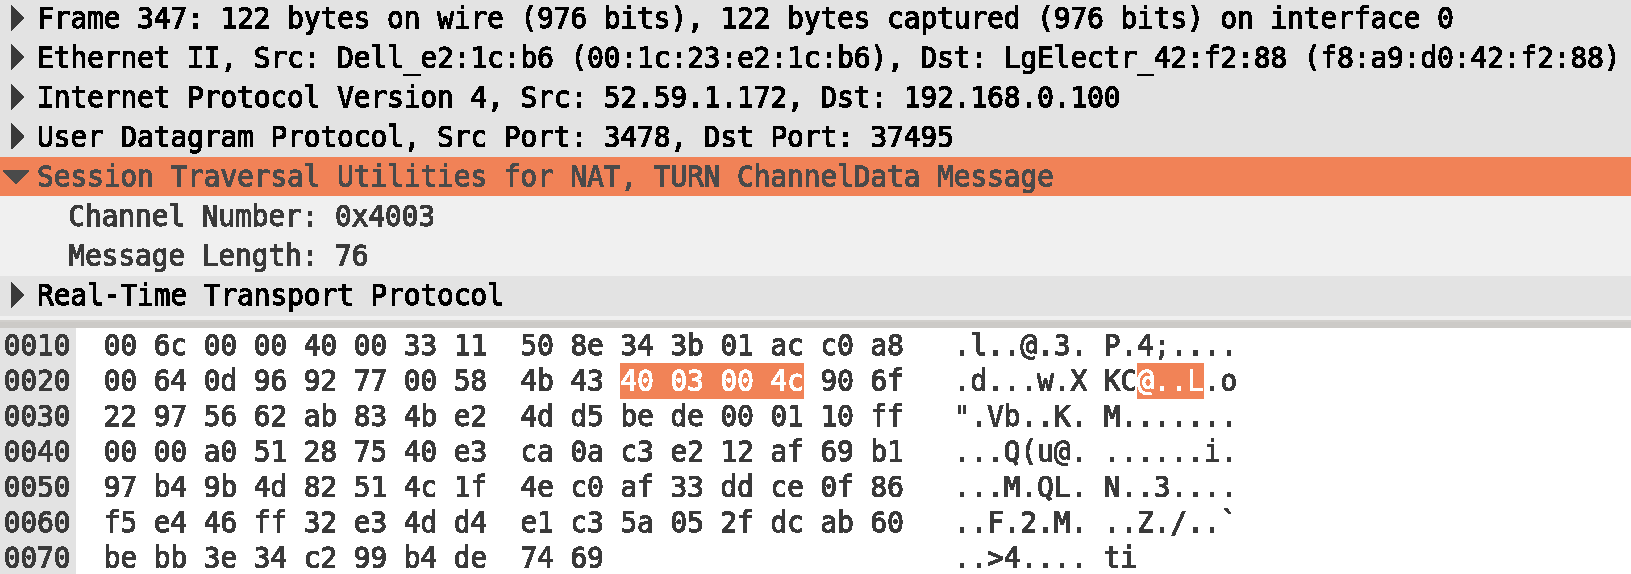
\includegraphics[width=.85\linewidth]{turn-channeldata}
	\caption{Ein Vektografik Screenshot}
	\label{fig:turn-channeldata}
\end{figure}

Falls möglich sollten stets Vektorgrafiken verwendet werden. Diese können zum Beispiel mit Visio erstellt und als PDF exportiert werden. Die PDF Datei kann dann in \LaTeX{} als Grafik verwendet werden. Der Code hierfür lautet wie folgt:

% the float option prevents figures to be placed in the listing but also prevents the listing from spanning multiple pages
\begin{lstlisting}[language=latex,float]
\begin{figure}
	\centering %Zentrieren
	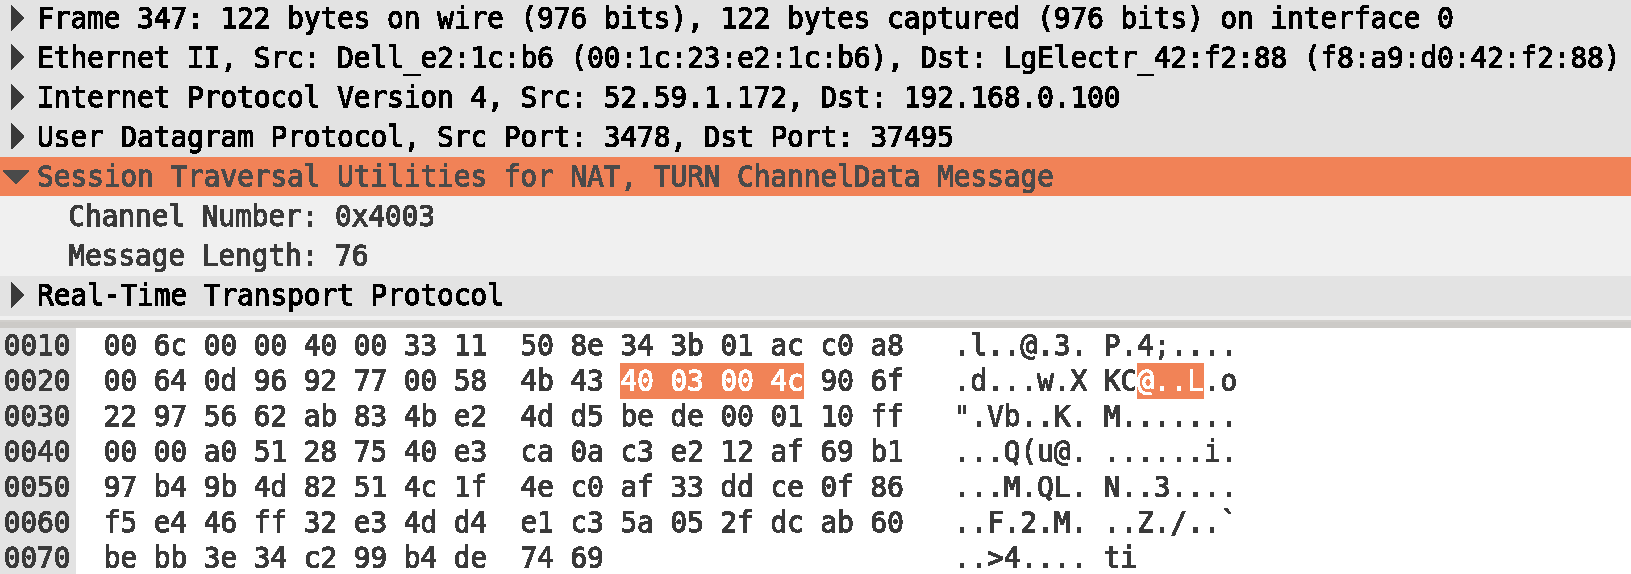
\includegraphics[width=.85\linewidth]{turn-channeldata} % Grafik einbinden (ohne Dateiendung) und auf 85 % der Seitenbreite Skalieren
	\caption{Ein Vektografik Screenshot} % Die Bildunterschrift
	\label{fig:turn-channeldata} % Das Label, mit dem die Grafik im Text referenziert werden kann
\end{figure}
\end{lstlisting}

Im Text kann ich auf eingebundene Abbildungen verweisen. In \autoref{fig:turn-channeldata} ist ein Vektorgrafik Screenshot zu sehen. Verwendet man \verb|\autoref{<label>}|, wird die Bezeichnung (Abbildung, Tabelle, Abschnitt\dots) automatisch ergänzt.


\begin{figure}[ht]
	\newcounter{density}
	\setcounter{density}{20}
	\centering
	\begin{tikzpicture}
	\def\couleur{cyan}
	\path[coordinate] (0,0)  coordinate(A)
	++( 90:5cm) coordinate(B)
	++(0:5cm) coordinate(C)
	++(-90:5cm) coordinate(D);
	\draw[fill=\couleur!\thedensity] (A) -- (B) -- (C) --(D) -- cycle;
	\foreach \x in {1,...,40}{%
		\pgfmathsetcounter{density}{\thedensity+20}
		\setcounter{density}{\thedensity}
		\path[coordinate] coordinate(X) at (A){};
		\path[coordinate] (A) -- (B) coordinate[pos=.10](A)
		-- (C) coordinate[pos=.10](B)
		-- (D) coordinate[pos=.10](C)
		-- (X) coordinate[pos=.10](D);
		\draw[fill=\couleur!\thedensity] (A)--(B)--(C)-- (D) -- cycle;
	}
	\end{tikzpicture}
	\caption{Rotated square from
		\href{http://www.texample.net/tikz/examples/rotated-polygons/}{texample.net}.}
	\label{fig:tikz1}
\end{figure}

Grafiken können auch direkt in \LaTeX{} mittles des TikZ Paketes erstellt werden (\autoref{fig:tikz1}). Auch verschiedenste Diagramme und Plots sind möglich (\autoref{fig:tikz2}). Zur vereinfachten Erstellung sind Tools, wie z.\,B. \href{https://www.mathcha.io}{https://www.mathcha.io} hilfreich.

\begin{figure}[ht]
	
	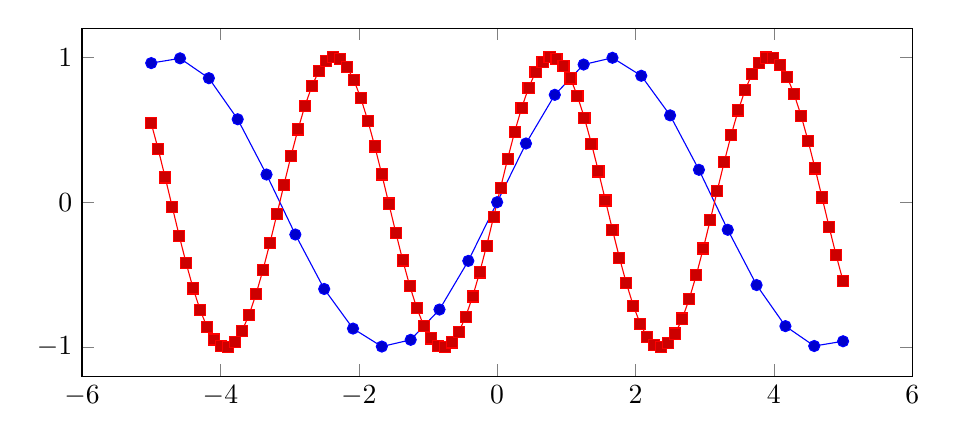
\begin{tikzpicture}
		\begin{axis}[
%		mlineplot,
		width=\textwidth,
		height=6cm,
		]
		
		\addplot {sin(deg(x))};
		\addplot+[samples=100] {sin(deg(2*x))};
		
		\end{axis}
	\end{tikzpicture}
	\caption{Ein Sinusplot mittels TiKZ}
	\label{fig:tikz2}
\end{figure}

\begin{figure}[ht]
	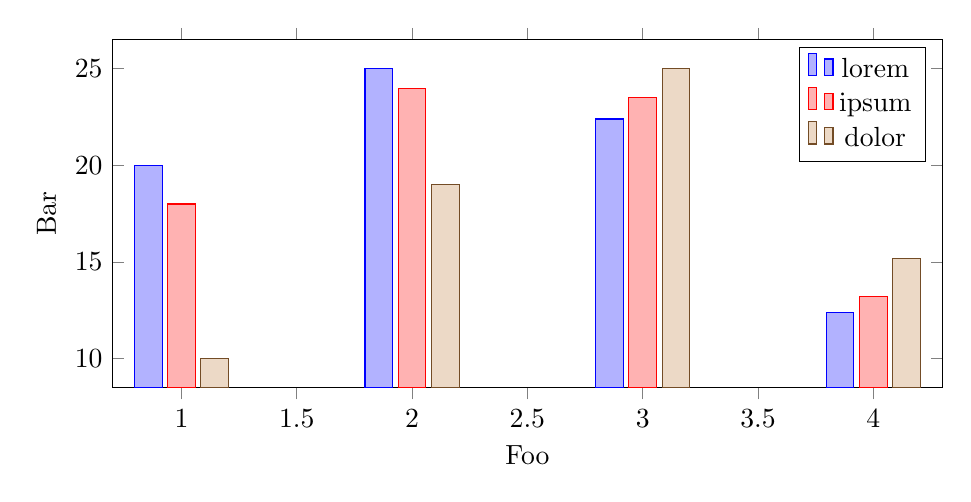
\begin{tikzpicture}
	\begin{axis}[
	ybar,
	xlabel={Foo},
	ylabel={Bar},
	width=\textwidth,
	height=6cm,
	]
	
	\addplot plot coordinates {(1, 20) (2, 25) (3, 22.4) (4, 12.4)};
	\addplot plot coordinates {(1, 18) (2, 24) (3, 23.5) (4, 13.2)};
	\addplot plot coordinates {(1, 10) (2, 19) (3, 25) (4, 15.2)};
	
	\legend{lorem, ipsum, dolor}
	
	\end{axis}
	\end{tikzpicture}
	\caption{Ein Balkendiagramm}
	\label{fig:tikz3}
\end{figure}

Wie in \autoref{fig:tikz3} zu sehen, sind auch Balkendiagramme möglich.

Mit \verb|\autoref{<label>}| kann man auch auf Abschnitte oder Kapitel verweisen. Im PDF wird automatisch eine Verlinkung hinzugefügt (siehe \autoref{sec:kommunikationsvorgange}).

\section{Tabellen}
\begin{otherlanguage*}{USenglish} % Switch document language temporarily but keep labels in main language. For better hyphenation! Use the unstarred variant to translate the labels as well.
\begin{table}
	\centering
	\caption[Modes of operation according to \glsentrytext{itu-t}]{Modes of operation according to \textcite{ITU-T.P.564}}
	\label{tab:modes_P.564}
	\begin{tabularx}{\textwidth}{@{}lclX@{}}
		\toprule
		\multicolumn{1}{c}{\textbf{Class}} & \textbf{Mode} & \multicolumn{1}{c}{\textbf{Name}} & \multicolumn{1}{c}{\textbf{Description}}                                                                            \\ \midrule
		\multirow{5}{*}{Midpoint}          & \multirow{2}{*}{A}             & \multirow{2}{*}{Dynamic operation}                 & The model uses information from RTCP-XR packets to optimize its prediction. \\ \cmidrule{2-4}
		& \multirow{2}{*}{B}             & \multirow{2}{*}{Static operation}                  & The model has been optimized or configured using \textit{a priori} knowledge of the endpoint.                                \\ \midrule
		\multirow{2}{*}{Endpoint}                            & \multirow{2}{*}{C}             & \multirow{2}{*}{Embedded operation}                & The model is co-located with the jitter buffer in the endpoint and has access to the jitter buffer.                 \\ \bottomrule
	\end{tabularx}

\end{table}
\end{otherlanguage*}
Tabellen können kompliziert in der Erstellung sein. Zum Glück gibt es Hilfsmittel wie den \enquote{\LaTeX{} Tables Generator}~\footnote{\href{https://www.tablesgenerator.com/}{https://www.tablesgenerator.com/}}. Dann ist auch die Erstellung von komplexeren Layouts wie in \autoref{tab:modes_P.564} kein Problem.


\section{Quellcode}
Auch Quellcode mit automatischem Syntaxhighlighting kann eingebunden werden. Die Referenzierung funktioniert auch hier (siehe \autoref{lst:signalexample}). Für noch schönere Quellcodelistings empfiehlt sich das Paket \href{https://ctan.org/pkg/minted?lang=de}{\texttt{minted}}, welches anstelle des \texttt{listings} Paket verwendet wird (Python benötigt!).
\begin{lstlisting}[language=c,caption={[Ein einfaches Quellcodelisting]Ein einfaches Quellcodelisting~\cite{wolf_LinuxsystemprogrammierenCKurs_2003}},label=lst:signalexample]
#include <stdio.h>
#include <stdlib.h>
#include <signal.h>

void sigfunc(int sig) {
	char c;
	if(sig != SIGINT)
		return;
	else {
		printf("\nWollen sie das Programm beenden (j/n) : ");
		c=getchar();
		if(c=='j')
			exit(0);
		return;
	}
}
int main() {
	int i;
	signal(SIGINT,sigfunc);
	while(1) {
	printf("Die Endlosschleife können sie mit STRG-C beenden");
	for(i=0;i<48;i++) {
		printf("\b"); //Cursor nach links bewegen
	}
	return 0;
}
\end{lstlisting}

\section{Sonstiges}
Es wird auch eine Umgebung für Beschreibungen bereitgestellt, bei denen das Label rechtsbündig ausgerichtet ist und die Beschreibung linksbündig. In die eckigen Klammern kommt das längste Label, damit \LaTeX{} die Abstände automatisch berechnen kann. Im Folgenden wird ein Beispiel für so eine Umgebung gebracht:

\begin{lstlisting}[language=latex,breaklines]
\begin{aligneddescription}[Registration success rate]
	\item[Registration success rate] describes the rate of successful registration attempts with the \ac{webrtc} signaling server.
	\item[Service availability] is defined in terms of capacity to establish calls from, and to \ac{webrtc} endpoints. 
	\item[Post dialing delay] is the time interval (in seconds) between the end of dialing by the caller and the reception back by him of the appropriate ringing tone or recorded announcement.
	\item[Call drop rate] equals service continuity in terms of capacity to maintain calls to their normal end.
\end{aligneddescription}
\end{lstlisting}
Das Ergebnis sieht wie folgt aus:
\begin{otherlanguage*}{USenglish} % switch to english hyphenation again
\begin{aligneddescription}[Registration success rate]
	\item[Registration success rate] describes the rate of successful registration attempts with the \ac{webrtc} signaling server.
	\item[Service availability] is defined in terms of capacity to establish calls from, and to \ac{webrtc} endpoints. 
	\item[Post dialing delay] is the time interval (in seconds) between the end of dialing by the caller and the reception back by him of the appropriate ringing tone or recorded announcement.
	\item[Call drop rate] equals service continuity in terms of capacity to maintain calls to their normal end.
\end{aligneddescription}
\end{otherlanguage*}

Des Weiteren bietet \KOMAScript{} die \texttt{labeling} Umgebung. Diese arbeitet ähnlich wie die \texttt{aligneddesription} Umgebung, jedoch sind die Labels linksbündig ausgerichtet. Das Ergebnis sieht wie folgt aus:

\begin{otherlanguage*}{USenglish} % switch to english hyphenation again
\begin{labeling}{Registration success rate}
	\item[Registration success rate] describes the rate of successful registration attempts with the \ac{webrtc} signaling server.
	\item[Service availability] is defined in terms of capacity to establish calls from, and to \ac{webrtc} endpoints. 
	\item[Post dialing delay] is the time interval (in seconds) between the end of dialing by the caller and the reception back by him of the appropriate ringing tone or recorded announcement.
	\item[Call drop rate] equals service continuity in terms of capacity to maintain calls to their normal end.
\end{labeling}
\end{otherlanguage*}

Hier zum Vergleich die Standard \texttt{description} Umgebung:

\begin{otherlanguage*}{USenglish} % switch to english hyphenation again
\begin{description}
	\item[Registration success rate] describes the rate of successful registration attempts with the \ac{webrtc} signaling server.
	\item[Service availability] is defined in terms of capacity to establish calls from, and to \ac{webrtc} endpoints. 
	\item[Post dialing delay] is the time interval (in seconds) between the end of dialing by the caller and the reception back by him of the appropriate ringing tone or recorded announcement.
	\item[Call drop rate] equals service continuity in terms of capacity to maintain calls to their normal end.
\end{description}
\end{otherlanguage*}

\section{Mathematik}
Auch mathematische Gleichungen können verwendet werden. In \autoref{eq:pam} ist ein Beispiel unter Verwendung der \texttt{equation} in Kombination mit der \texttt{split} Umgebung zu sehen. Damit können lange Gleichungen an bestimmten stellen umgebrochen und ausgerichtet werden.

\begin{equation}\label{eq:pam}
\begin{split}
f_{PAM_{M}}(t) = A_{T}\cdot \dfrac{T_{i}}{T_{T}} \Bigg[ 1+& \dfrac{A_{M}}{A_{T}}\cdot \mathrm{si}\left(f_{M}\cdot T_{i}\cdot \pi \right) \cdot \cos{\omega_{M}t} + \\
& \sum _{n=1}^{\infty }2\cdot \mathrm{si}\left(n\cdot f_{T}\cdot T_{i} \cdot \pi \right)\cos{\left(n\cdot \omega_{T} t \right)}  +  \\
& \sum _{n=1}^{\infty } \dfrac{A_{M}}{A_{T}} \cdot \mathrm{si}\left((n\cdot f_{T} + f_{M}) \cdot T_{i} \cdot \pi \right)\cos{\left(n\cdot \omega_{T} + \omega_{M}\right)}t +  \\
& \sum _{n=1}^{\infty } \dfrac{A_{M}}{A_{T}} \cdot \mathrm{si}\left((n\cdot f_{T} - f_{M})\cdot T_{i} \cdot \pi \right)\cos{\left(n\cdot \omega_{T} - \omega_{M})t\right)} \Bigg]
\end{split}
\end{equation}

Auch Gleichungen können mit einem Label versehen werden und mittels \lstinline[language=latex]|\autoref{<label>}| im Text referenziert werden. Siehe \autoref{eq:snr}. Der nachfolgende Code ergibt \autoref{eq:snr} und kann mittels \lstinline[language=latex]|\autoref{eq:snr}| referenziert werden:

\begin{lstlisting}[language=latex,breaklines]
\begin{equation}\label{eq:snr}
SNR(\si{\decibel}) = 10 \cdot \log_{10}\Bigg(\dfrac{P_{S}}{P_{R}} \Bigg)
\end{equation}
\end{lstlisting}

\begin{equation}\label{eq:snr}
	SNR(\si{\decibel}) = 10 \cdot \log_{10}\Bigg(\dfrac{P_{S}}{P_{R}} \Bigg)
\end{equation}

Auch der Umgang mit Einheiten ist dank des \texttt{siunitx} Paketes sehr einfach. So wird beispielsweise aus \lstinline[language=latex]|\SI{24.06}{\kilo\bit\per\second}|: \SI{24.06}{\kilo\bit\per\second} und aus \lstinline[language=latex]|\SIrange{20} {20000}{\hertz}|: \SIrange{20}{20000}{\hertz}.

% Include the other chapters
% !TeX root = ../my-thesis.tex
\chapter{Einleitung}
\section{Thematische Einführung}
Mobile Gräte wie Smartphones oder Tablets sind aus dem heutigen Alltag der Menschen nicht mehr wegzudenken. Ob zur privaten Unterhaltung beim spielen aufwendiger 3D Spiele, streamen von Musik- und Videoinhalten oder als unentbehrliches Werkzeug bei der täglichen Arbeit, mobile Geräte sind nahezu den gesamten Tag im Einsatz. Auch die Außendiensttechniker der DT Technik GmbH nutzen mobile Applikationen wie die Bestell-App oder die Mess-App zur Verwaltung und Aufstockung ihrer Werkzeuge und Ersatzteile beziehungsweise zur Untersuchung und Konfiguration von Routern. Hohe Akkulaufzeiten sind für diese Art der Benutzung eine Voraussetzung und stellen Smartphone Hersteller sowie Softwareentwickler vor die Herausforderung energieeffiziente Lösungen zu finden.
Dabei werden verschiedene Ansätze verfolgt. Auf der einen Seite versuchen die Hersteller energiesparende Prozessoren und Displays zu entwickeln und die Hardwarenutzung zu optimieren. Dieses Bestreben steht jedoch im Konflikt mit den Wünschen der Kunden, welche schnellere Mehrkern Prozessoren und größere Displays für die neuen Geräte erwarten. Dieser Trend ist auch in der Marktentwicklung der letzten zehn Jahre zu beobachten. So entsprach die durchschnittliche Displaygröße 2009 c.a. 3,2 Zoll. Acht Jahre später waren bereits Displays mit 5,5 Zoll üblich.\todo{Quellen Displaygröße} Auf der anderen Seite versuchen Anwendungsentwickler durch Softwareoptimierung ihre Applikationen ressourcensparender zu gestalten. Dabei können Prozesse wie zum Beispiel größere Downloads für Datenbankupdates als Service oder mithilfe des neuen Android Work Manager's als Hintergrundprozess implementiert werden und in Abhängigkeit vom aktuellen Ladestand des Akkus auf günstigere Zeitpunkte verschoben werden.\todo{Quelle WorkManager} Auch das gewissenhafte Umgehen mit Wake Locks und das festlegen der Standby Phasen der eigenen Applikation sind wichtige Stellschrauben, über welche ein Anwendungsentwickler energiesparende Anpassungen justieren kann.\todo{Quelle Appstandby und Wake locks} Dies sind nur einige Beispiele  der möglichen Optionen für Energieoptimierungen auf mobilen Geräten. Das Problem der Energieeffizienz auf mobilen Geräten bietet ein breites Feld an Forschungspotential und wird auch zukünftig eine zentrale Rolle in der Geräteherstellung und App-Entwicklung spielen.
\section{Thematische Abgrenzung und Zielstellung dieser Arbeit}
In dieser Arbeit werden verschiedene Implementierungsansätze für Algorithmen und Berechnungen betrachtet und auf deren Einfluss auf den Energieverbrauch mobiler Geräte untersucht. Der Schwerpunkt liegt hierbei auf der Betrachtung von parallelen Berechnungen mithilfe von Multithreading. Dabei wird der Zusammenhang zwischen der Anzahl der parallel laufenden Threads, der Laufzeitveränderung und dem damit einhergehenden Energieverbrauch gemessen.
Ziel dieser Untersuchung ist es, herauszufinden ob es einen Zusammenhang zwischen den drei genannten Parametern gibt und gegebenenfalls eine Empfehlung für die Implementierung von Multithreading herauszuarbeiten, welche einen sinnvollen Kompromiss aus Laufzeit und Energieverbrauch bereitstellt.
Weiterhin wird der Unterschied zwischen rekursiven und iterativen Implementierungen hinsichtlich des Stromverbrauchs betrachtet. Auch hier ist das Ziel, die ressourcenschonendste Variante zu ermitteln.


\section{Struktureller Aufbau und Vorgehensweise der Untersuchung}

Das anschließende Kapitel \glqq Untersuchte Konzepte und Implementierungen\grqq{} beschreibt die theoretischen Aspekte von paralleler Programmierung und deren Einfluss auf den Energieverbrauch sowie die für diese Arbeit relevanten Gesetzmäßigkeiten und Berechnungsformeln des Multiprocessings. Außerdem werden die zur Untersuchung entwickelten Implementierungen vorgestellt, welche in der \glqq EnergyEfficience\grqq{} Applikation angewandt werden. Für die Umsetzung einer parallelen Ausführung wurde ein Base64 Encoder implementiert. Dieser ist nur ein Mittel zum Zweck und könnte durchaus durch andere lineare Algorithmen ersetzt werden. Des Weiteren werden auch die Unterschiede von rekursiven und iterativen Algorithmen beleuchtet und gegenübergestellt, da diese den zweiten großen Untersuchungsgegenstand dieser Arbeit bilden. Weil der Merge Sort Algorithmus aufgrund seiner Vielseitigkeit perfekt für die Gegenüberstellung dieser beiden Implementierungsstrategien geeignet ist, werden in diesem Kapitel die verwendeten Merge Sort Varianten inklusive ihrer Implementierung dargestellt.

Im folgenden Kapitel 3 \glqq Verwendete Geräte und Tools\grqq{} werden alle Programme und Geräte samt deren Spezifikationen vorgestellt, die im Rahmen dieser Untersuchung genutzt wurden. Es wird eine kurze Einführung in die Verwendung des Programms Battery Historian geben. Weiterhin wird die eigens für diese Arbeit entwickelte App vorgestellt. Anschließend wird die Messmethode mithilfe dieser beiden Tools beschrieben.

In Kapitel 4 \glqq Energieeffizientes Multithreading\grqq{} werden die Ergebnisse der Messungen des parallelen Base64 Encoders dargestellt und ausgewertet. Der Fokus liegt hierbei auf dem Zusammenhang zwischen verwendeter Thread-Anzahl und Energieverbrauch.

Daraufhin untersucht Kapitel 5 \glqq Rekursive und Iterative Verfahren im Vergleich\grqq{} den Einfluss von iterativer beziehungsweise rekursiver Implementierung auf den Energieverbrauch. Hierfür wird die bereits erwähnte Merge Sort Implementierung der \glqq EnergyEfficience\grqq{} Applikation genutzt. Außerdem werden die Vorzüge des Fork-Join Thread Pools bei paralleler Rekursion durch Messungen untersucht..

Im abschließenden Kapitel 6 \glqq Auswertung\grqq{} ist eine Zusammenfassung der gewonnen Erkenntnisse zu finden. Außerdem werden im Ausblick Ansätze für weitere Untersuchungen auf diesem Gebiet formuliert.


% !TeX root = ../my-thesis.tex
\chapter{Untersuchte Konzepte und Implementierungen}

\section{Theoretische Aspekte in die Parallelität}
Das Ziel hinter der Parallelisierung von Aufgaben ist die Beschleunigung der Laufzeit bei der Abarbeitung von Programmabläufen und die Minimierung der Wartezeiten des Prozessors. Solche Wartezeiten können entstehen, wenn während der Programmausführung Benutzereingaben nötig sind bevor die Ausführung fortgesetzt werden kann oder wenn neue Daten aus dem vergleichsweise langsamen Hauptspeicher nachgeladen werden müssen, da der prozessoreigene Cache nicht groß genug ist \cite[1135]{wolf2020}. Ohne Parallelität würden moderne Softwareanwendungen jeglicher Art nahezu unnutzbar werden. Einfache Vorgänge wie das Laden von Benutzerdaten aus einer lokalen Datenbank oder das downloaden von Bildern aus dem Netz, würden zum Einfrieren der Benutzeroberfläche führen, da bei sequentiellen Programmabläufen alle Aufgaben strikt hintereinander ausgeführt werden müssen. Android selbst wäre ohne Parallelität nicht umsetzbar, da Android's Architektur Multithreading und damit Parallelität voraussetzt.\todo{Erklärung}

Für die Realisierung von Parallelität haben sich mit der Evolution der Prozessortechnologie verschieden Ansätze und Techniken entwickelt. Jede dieser Techniken ist bis heute relevant und glänzt in unterschiedlichen Anwendungsfällen.

\underline{Pipelining}

Beim Pipelining wird die Ausführung von Befehlen in verschiedene Phasen aufgeteilt, welche jeweils durch eine eigene Ausführungseinheit bearbeitet werden. Sobald ein Befehl die aktuelle Phase abgeschlossen hat und zur nächsten Phase springt, kann bereits mit der Bearbeitung des nächsten Befehls, in der frei gewordenen Phase begonnen haben. In \autoref{fig:Pipeline} ist ein Beispiel einer 5-Phasen Pipeline veranschaulicht. Die Bearbeitung jeder Phase dauert im Optimalfall einen Taktzyklus, da andernfalls die Pipeline durch dies Phase geblockt werden kann, wie es in diesem Beispiel bei Befehl 3 während der Execute Phase der Fall ist. Ein großer Nachteil von Pipelining tritt bei häufigen Programmsprüngen auf, da bei jedem Sprung die komplette Pipeline geleert werden muss und alle Phasen, die bis dorthin vollendet wurden, verworfen werden und umsonst bearbeitet wurden. Dieser ist besonders bei größeren Pipelines kritisch \cite{pipelineElektro}.
\begin{figure}[H]
	\begin{center}	 
	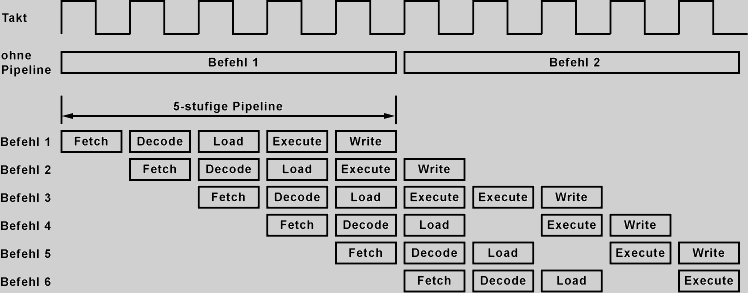
\includegraphics[scale=1]{Pipeline}
	\caption{Beispiel für eine 5-Phasen-Pipeline (Quelle: \cite{pipelineElektro})}
	\label{fig:Pipeline} 
	\end{center}
\end{figure}

\underline{simultanes Multi-Threading}

Ein Thread ist ein sequenzieller Ausführungspfaden innerhalb eines Prozesses, der ausgeführt wird. Bei Rechnern mit einem Prozessor kann zu einem Zeitpunkt immer nur ein Thread eines Prozesses gleichzeitig ausgeführt werde. Falls dieses Ausführung durch Ereignisse wie Speicherzugriffe oder Nutzereingaben warten muss, blockiert dieser Thread die \ac{cpu}. Durch sogenanntes simultanes Multi-Threading wird die verfügbare \ac{cpu} Zeit auf mehrere Prozesse und Threads aufgeteilt. Die \ac{cpu} kann dadurch zwischen den Threads hin und her springen und so längere Wartezeiten verhindern. Dies steigert die Effizienz der \ac{cpu} hinsichtlich der Laufzeit sowie des Energieverbrauchs \cite[877]{cplusplus}.

\underline{Hyper-Threading}

Die Technologie Hyperthreading wurde von Intel mit den Prozessoren Pentium 3, Pentium 4 und Xeon eingeführt. Hierbei wird wird der Durchsatz von Multithreaded-Anwendungen im Multitasking erhöht, indem sie die Auslastung der On-Chip-Ressourcen erhöht, die in der Intel-NetBurst-Mikroarchitektur verfügbar sind. Ein typischer Thread belastet nur etwa 35 \% der NetBurst-Ausführungsressourcen. Hyperthreading erhöht die Auslastung durch notwendige Logik und Ressourcen, die der CPU hinzugefügt werden. Für die Aufteilung der einkommenden Daten auf den freien Raum sorgen somit zwei logische Prozessoren, die vom Betriebssystem mittels klassischer Multiprocessing-Verfahren verwaltet werden \cite[1138]{wolf2020}. Somit stehen dem Rechner also 2 logische Rechenkern zur Verfügung trotz physischer Single Core \ac{cpu}. Dies bietet die Möglichkeit Speicherwartezeiten zu überbrücken. Wenn der erste Thread im Wartezustand ist, kann der Prozessor mithilfe des zweiten logischen Kerns in der Programmausführung fortfahren.

\underline{Multi-Core-Prozessor}

Bei Multi-Core Systemen handelt es sich um Prozessoren mit mehreren physischen Rechenkernen. Diese können voneinander unabhängig arbeiten und ermöglichen echte Parallelität. Alle Rechenkerne nutzen auch die schon genannten Techniken um möglichst effiziente Ergebnisse zu erhalten. Der Vorteil liegt hierbei nicht nur in der Steigerung der Geschwindigkeit. Mehrkernprozessoren können wesentlich geringer getaktet werden als Single Core Prozessoren und ermöglichen trotzdem erhöhte Laufzeitgeschwindigkeit bei geringerer Leistungsaufnahme und Wärmeentwicklung \cite{MulicoreElektro}. Es könnte die Annahme getroffen werden, dass mit steigender Rechenkernzahl auch die Leistung addiert wird. Sodass die neue Laufzeit im Multi-Core-Betrieb gleich der ursprünglichen Laufzeit mit einem Kern geteilt durch die Anzahl der Rechenkerne beträgt. In der Realität ist dies jedoch nicht umsetzbar, da verschiedene Faktoren diese Annahme begrenzen. Zunächst einmal wächst mit steigender Anzahl an Rechenkernen auch der Aufwand der Verwaltung durch das Betriebssystem. Außerdem ist es nicht einfach den Zugriff auf geteilte Speicherressourcen durch mehrere Rechenkerne zu synchronisieren. Die Laufzeit für parallele Prozesse setzt sich grob aus folgenden Anteilen zusammen.
\begin{aligneddescription}
\item[Rechenzeit] Zeit für die Durchführung von Berechnungen unter Verwendung von Daten im lokalen Speicher der einzelnen Prozessoren.
\item[Kommunikationszeit] Zeit für den Austausch von Daten zwischen Prozessoren.
\item[Wartezeit] Z.B. aufgrund ungleicher Verteilung von Last zwischen den Rechenkernen, Datenabhängigkeiten im Algorithmus oder Ein- und Ausgabe.
\item[Synchronisationszeit] Zeit für die Synchronisation beteiligter Prozesse und von Ressourcenzugriffen.
\item[Platzierungszeit] Zeit für die Allokation der Tasks auf die einzelnen Prozessoren, sowie eine mögliche dynamische Lastverteilung zur Programmlaufzeit.
\item[Startzeit] Zeit zum Starten der parallelen Threads auf allen Rechenkernen.
\end{aligneddescription}\cite[313]{parallelBook}

Viele Anwendungen können nur für kleine Bestandteile ihrer Ausführung von den Vorteilen eines Multi-core Systems profitieren, da die meisten Anwendungsfälle durch Nutzeraktionen bestimmt sind. Bei Programmabläufen mit strikt aufeinanderfolgenden Abhängigkeiten ist Parallelität ohnehin nicht möglich und resultiert in traditionell sequentielle Abläufe. Das Admahl'sche Gesetz beschreibt genau diese Grenze. So ist der Beschleunigungsfaktor, auch Speedup genannt, mit zusätzlichen Rechenkernen durch sequentielle Anteile eines Problems begrenzt \cite[314]{parallelBook}. Das Admahl'sche Gesetz, benannt nach Gene Admahl, dient zur Vorhersage der maximal zu erwartenden Beschleunigung eines Algorithmus durch parallele Ausführung und wird wie folgt beschrieben.

\begin{aligneddescription}
\item[Speedup] Beschleunigungsfaktor der Rechenzeit durch $p$ Kerne ($S_{p}(n)$)
\item [sequentielle Laufzeit] Laufzeit bei Ausführung mit einem Rechenkern ($T_{seq}(n)$)
\item[Anzahl der Rechenkerne] Anzahl der an der parallelen Ausführung beteiligten Prozessorkernen ($p$)
\item[sequentieller Anteil] Anteil des Problems, welcher ausschließlich sequentiell ausführbar ist ($f$). Es gilt $0\leq f \leq 1$ wobei $f = 1$ bedeuteten würde, dass das gesamte Problem, also 100 \% des Problems, sequentiell ausgeführt werden muss.
\item[paralleler Anteil] Anteil des Problems, welcher parallelisierbar ist ($(1-f)$)
\item[parallele Laufzeit] Laufzeit bei paralleler Ausführung mit $p$ Rechenkernen für ein Problem der Größe $n$ ($T_{p}(n)$)
\item[Problemgröße] Die Größe der Berechnung des Algorithmus ($n$)
\end{aligneddescription}
\begin{equation}\label{eq:Amdahlsche Gesetz}
S_{p}(n)=\frac{T_{seq}(n)}{T_{p}(n)} =
\frac{T_{seq}(n)}{f*T_{seq}(n) + \frac{ (1-f)*T_{seq} }{p}}
\end{equation}
\cite[317]{parallelBook}

Der Speedup $S_{ p }(n)$ wird aus \autoref{eq:Amdahlsche Gesetz} wird im Rahmen dieser Arbeit für die Ermittlung der Effizienz es Multithreadings benötigt, welche wie folgt beschrieben ist. 
\begin{equation}\label{eq:Effizienz}
E_{ p }(n) =\frac{ S_{ p }(n) }{p}
\end{equation}
\cite[316]{parallelBook}
Die Effizienz (\autoref{eq:Effizienz}) eines parallelen Programms gibt die relative Verbesserung des Speedups $S_{ p }(n)$ bezüglich der Anzahl $p$ der Prozessorkerne an. Diese Größe wird im Laufe dieses Kapitels für den Vergleich von Laufzeiteffizienz und Energieeffizienz in Abhängigkeit der Thread Anzahl verwendet.

\section{Thread Pool Implementierung in Android}

Die \glqq EnergyEfficience\grqq{} App wurde vollständig in Java entwickelt. An dieser Stelle sei erwähnt, dass mit der immer stärkeren Kotlin Auslegung des Android Frameworks neue Technologien hinsichtlich Multithreading und Synchronisation an Beliebtheit gewinnen. Kotlin bietet neben den traditionellen Java Techniken wie Threading, Callbacks und Futures auch sogenannte Kotilin Corountines. Durch Corountines können Ausführungen von längeren Funktionen beliebig pausiert werden, um anschließend mit anderen Aufgaben fortzufahren. Sobald die \ac{cpu} wieder freie Ressourcen hat, springt die der Programmcounter an die Stelle der pausierten Funktion zurück und nimmt die Ausführung wieder auf. Dies verhindert blockierende Berechnungen, welche beispielsweise zur Einfrierung der \ac{ui} führen können. Hierbei reicht es das Schlüsselwort \glqq suspend\grqq{} bei der Deklaration der Funktion anzugeben. Verglichen mit der Implementierung von Callbacks ist diese Herangehensweise sehr einfach und schnell umzusetzen \cite{kotlin-corountines}. In Java wird Nebenläufigkeit traditionell mit der java.lang.Thread Klasse realisiert. Im  Konstruktor des Thread-Objekts wird eine Referenz auf ein Objekt vom Typ Runnable verlangt, welches den parallel auszuführenden Programmcode enthält. Das Runnable-Objekt implementiert diesen Code in der vom Rnnable-Interface definierten Methode run(). Bei der Nutzung ist es wichtig, den Code nicht einfach durch Aufruf dieser run()-Methode zu starten. Dies würde zu einer normalen sequentiellen Ausführung führen. Um eine parallele Ausführung zu erreichen muss die start()-Methode des entsprechenden Thread-Objekts aufgerufen werden. Dadurch wird für diesen Thread eine eigene Ablaufumgebung mit den nötigen Systemressourcen erstellt und automatisch die interne run()-Methode mit der Implementierung des Runnable-Objekts ausgeführt. Sobald die run()-Methode terminiert, wird der Thread automatisch beendet und seine Systemressourcen werden freigegeben. Es außerdem möglich eine eigene Klasse zu erstellen, die von Thread erbt und den auszuführenden Code direkt in der eigenen run()-Methode implementiert. Diese Variante ist jedoch weniger flexibel als das Benutzen von separaten Runnable-Objekten, da für jedes Problem eine erweiterte Thread-Klasse mit der entsprechenden run()-Methode erstellt werden müsste.  Bei der Ausführung von mehreren Threads zur gleichen Zeit, ist die Terminierung der Threads selbst bei identischen Aufgaben nicht vorhersehbar, da der Kontextwechsel zwischen parallellaufenden Threads vom Scheduler des Betriebssystems organisiert wird und daher nicht nachvollziehbar ist \cite{javaistauchnurInsel}. Generell muss erwähnt werden, dass die \ac{jvm} die Thread-Verwaltung direkt auf das Betriebssystem abbildet. Das bedeutet, dass die eigentliche Thread-Verwaltung inklusive der einhergehenden Ressourcenverwaltung nicht direkt durch die Java Implementierung beeinflusst werden kann sondern allein durch das zugrunde liegende Betriebssystem abgewickelt wird \cite{javaistauchnurInsel} \todo{Quelle Anpassen}. Sprachen wie C++ oder C sind für solche Aufgaben besser geeignet und ermöglichen einen Maschinennäheren Zugriff und dadurch potentiell performantere Lösungen.

Das Prinzip der Erstellung von Threads und der Kapselung des Ausführungscodes durch Runnables ist zwar die Grundlage für Multithreading in Java, reicht für die effektive Umsetzung von Threadpools jedoch nicht aus. Die feste Bindung zwischen dem Ausführungs-Thread und dem Runnable-Objekt ist zu unflexible um ein effizientes und benutzerfreundliches Thread-Management zu realisieren. Schon bei der Erzeugung eines Threads muss das Runnable-Objekt im Thread-Konstruktor übergeben werden und kann im Nachhinein nicht mehr geändert werden. Des Weiteren ist es nicht möglich die start()-Methode eines Threads mehrmals hintereinander aufzurufen, da dies zu einer Exeption führen würde falls der Thread bereits läuft. Weil das Thread-Objekt nach Abarbeitung des Runnables beendet und verworfen wird, ist es außerdem nicht möglich, Threads wiederzuverwenden. Das bedeutet, dass für jede Abarbeitung eines Raunnables ein neues Thread-Objekt erstellt werden muss. Selbst wenn die abzuarbeitende Aufgabe identisch ist muss ein neues Objekt mit dem gleichen Runnable instanziiert werden. Das ständige erstellen und verwerfen von Thread-Objekten führt zu einer permanenten Belastung des Garbage Collectors und kann zu Performance-Verlust führen. Um diese ungünstigen Nebenerscheinungen der starren Kopplung von Thread und Runnable-Objekt zu umgehen, bietet Java die Schnittstelle \emph{Executor}, welche die Ausführung des Runnable-Programmcodes von der Initialisierung der Threads trennt. Dieses Interface schreibt die Methode \emph{execute(Runnable command)} vor,  mit der die klassischen Runnables später ausgeführt werden. Für die Umsetzung des parallelen Base64-Encoders wurde ein Thread Pool Manager mithilfe der \emph{ThreadPoolExecutor} Klasse umgesetzt. \emph{ThreadPoolExecutor} ist eine Java eigene Implementierung der Schnittstelle \emph{Executor} um eine Sammlung von Threads aufzubauen, welche beliebig viele  Aufgaben (Runnables) koordiniert abarbeiten kann. Dabei werden den Threads ohne Aufgabe neue Runnables aus einer Aufgaben-Queue dynamisch zugeordnet \cite{javaistauchnurInsel}. Der \autoref{lst:CustomThreadManager} zeigt die Implementierung des \emph{ CustomThreadPoolManagers} in der \glqq EnergyEfficience\grqq{} App. Im Konstruktor wird eine Instanz des \emph{ThreadPoolExecutors} initialisiert. Mit \emph{NUMBER\_OF\_CORES} wird die maximale Anzahl der gleichzeitigen Worker-Threads angegeben. Standardmäßig wird dieser Wert durch Aufruf der Methoden \emph{Runtime.getRuntime().availableProcessors()} mit der Anzahl der physischen Rechenkerne des Gerätes gleichgesetzt. Da die Untersuchung jedoch unter Anderem darauf abzielt, das Verhalten des Energieverbrauchs bei variabler Anzahl von Worker-Threads darzustellen, gibt es eine  \emph{ setNumberOfCores(int numberOfCores)} Methode um  diesen Wert während der Laufzeit anzupassen. Die \emph{ KEEP\_ALIVE\_TIME} Variable legt fest, wie lange ein Thread ohne Aufgaben am Leben erhalten wird, um auf neue Runnables zur Ausführung zu warten. Bekommt der Thread innerhalb dieser Zeit keine neue Aufgabe zugewiesen, so werden seine Ressourcen für andere Prozesse freigegeben. Über eine \emph{ BlockingQueue} (\emph{mTaskQueue}) werden die vom Thread-Pool abzuarbeitenden Runnables zwischengespeichert. Dies ist eine spezielle Datenstruktur, die Operationen unterstützt, welche nicht sofort ausgeführt werden können. So könnte es zum Beispiel vorkommen, dass ein Thread aus dem Thread-Pool mit der letzten Ausführung fertig ist und nun nach einer weiteren Aufgabe fordert, ohne dass neue Runnables in der \emph{ mTaskQueue} vorhanden sind. Die \emph{ BlockingQueue} bietet hierfür die  poll(time, unit)-Methode. Dadurch wird der aufrufende Thread für den angegebenen Zeitraum geblockt, in welchem er auf neue Aufgaben in Form von Runnables wartet \cite{BlockingQueue}. Dieses Zeitintervall wird in \autoref{lst:CustomThreadManager} durch die Variablen \emph{ KEEP\_ALIVE\_TIME} und \emph{ KEEP\_ALIVE\_TIME\_UNIT} festgelegt. Da es mit normalen Runnables nur schwer möglich ist, Ergebnisse einer asynchronen Methodenausführung abzugreifen, wurden die Callables eingeführt. Callable-Objekte funktionieren ähnlich wie Runnable-Objekte und können daher auch wie Runnables behandelt werden. Allerdings implementieren sie statt der run()-Methode die call()-Methode. Wenn ein Callable-Objekt durch \emph{submit(Callable c)} der \emph{ mTaskQueue} hinzugefügt wird, dann  liefert  dieser Aufruf ein Objekt vom Typ \emph{Future}. Dieses Future-Objekt dient als Platzhalter für das zukünftige Ergebnis des asynchronen Aufrufs.  In der Methode \emph{ addCallable(Callable callable)} werden neue Aufgaben in Form von Callables der \emph{ mTaskQueue} hinzugefügt und gleichzeitig Future-Objekte für jedes dieser Callalbes in die \emph{ mTaskQueue} geschrieben. Mit dieser Struktur ist ein eleganter Zugriff auf die Ergebnisse der asynchronen Thread-Ausführungen möglich, ohne dabei die eigentliche Routine der Threads zu stören. Um zu verhindern, dass mehrere Instanzen dieses Thread-Pools gleichzeitig existieren können, wurde diese Klasse als sogenanntes Singleton implementiert. Singleton ist die Bezeichnung für ein Design Pattern aus der Softwareentwicklung, bei dem sichergestellt wird, dass von einer Klasse nur eine einzige Instanz existiert. Diese Instanz wird global definiert, sodass es an jeder Stelle im Projekt verfügbar ist.  Zur Umsetzung wurde der Konstruktor als \emph{private} definiert, um zu verhindern, dass weitere Instanzen außerhalb des Klassenkontextes erstellt werden können. In Zeile 14 von \autoref{lst:CustomThreadManager} wird einmalig eine statische Instanz von \emph{CustomThreadPoolManager} definiert, welche durch die statische Klassenmethode \emph{getInstance()} abrufbar ist. Die \emph{BackgroundThreadFactory} wird benötigt um die Erstellung und Zuweisung von neuen Threads mit Runnable-  beziehungsweise Callable-Objekten zu automatisieren.

\begin{lstlisting}[language=java,caption={der CustomThreadManager aus der EnergyEfficience App},label=lst:CustomThreadManager]
public class CustomThreadPoolManager {

    private  static int NUMBER_OF_CORES = Runtime.getRuntime().availableProcessors();
    private static final int KEEP_ALIVE_TIME = 1;
    private  static final TimeUnit KEEP_ALIVE_TIME_UNIT;
    private Handler mainThreadHandler = HandlerCompat.createAsync(Looper.getMainLooper());
    private final ExecutorService mExecuterService;
    private final BlockingQueue<Runnable> mTaskQueue;
    private List<Future> mRunningTaskList;
    private static CustomThreadPoolManager singleInstance = null;

    static{
        KEEP_ALIVE_TIME_UNIT = TimeUnit.SECONDS;
        singleInstance = new CustomThreadPoolManager();
    }
    private CustomThreadPoolManager(){
        mTaskQueue = new LinkedBlockingQueue<Runnable>();
        mRunningTaskList = new ArrayList<>();
        mExecuterService = new ThreadPoolExecutor(
                NUMBER_OF_CORES,
                NUMBER_OF_CORES,
                KEEP_ALIVE_TIME,
                KEEP_ALIVE_TIME_UNIT,
                mTaskQueue,
                new BackgroundThreadFactory());
    }
    public static void setNumberOfCores(int numberOfCores) {
        if(numberOfCores > 0){
            NUMBER_OF_CORES = numberOfCores;
            singleInstance = new CustomThreadPoolManager();
        }
    }
    public void addCallable(Callable callable){
        Future future = mExecuterService.submit(callable);
        mRunningTaskList.add(future);
    }
    public Handler getMainThreadHandler(){
        return this.mainThreadHandler;
    }
    public static CustomThreadPoolManager getInstance(){
        return singleInstance;
    }
    public int getNumberOfCores(){
        return NUMBER_OF_CORES;
    }
    public void cancelAllTasks() {
        synchronized (this) {
            mTaskQueue.clear();
            for (Future task : mRunningTaskList) {
                if (!task.isDone()) {
                    task.cancel(true);
                }
            }
            mRunningTaskList.clear();
        }
    }
    private static class BackgroundThreadFactory implements ThreadFactory {
        private static int sTag = 1;
        @Override
        public Thread newThread(Runnable runnable) {
            Thread thread = new Thread(runnable);
            thread.setName("CustomThread" + sTag);
            sTag++;
            thread.setPriority(THREAD_PRIORITY_BACKGROUND);
            thread.setUncaughtExceptionHandler(new Thread.UncaughtExceptionHandler() {
                @Override
                public void uncaughtException(Thread thread, Throwable ex) {
                    Log.e("ThreadFactory", thread.getName() + " encountered an error: " + ex.getMessage());
                }
            });
            return thread;
        }
    }
}
\end{lstlisting}

\todo{handler Looper}
Die Flexibilität dieses Thread-Pools, der in der variablen Festlegung der Arbeiter Threads liegt bildet die Grundlage der folgenden Messungen. Ziel ist es, herauszufinden, welche Anzahl von Threads am energieeffizientesten ist und welcher Zusammenhang mit der Laufzeit besteht.

\section{Ein paralleler Base64 Encoder}

Für die Untersuchung der parallelen Ausführung über beliebig viele Threads wurde die Base64-Kodierung gewählt. Hierbei werden 8-Bit Binärdateien in eine 7-Bit-\ac{ascii}-Textrepräsentation umgewandelt. So können binäre Dateiformate wie beispielsweise Bilddateien in \ac{ascii}-Textformate umgewandelt werden und direkt in \ac{html}- oder \ac{css}-Dateien eingebunden werden. Auch für das Verschicken von E-Mails mit Anhang wird die Base64-Kodierung noch häufig genutzt, da \ac{smtp} ursprünglich nur in der Lage war, sieben-Bit-\ac{ascii}-Texte zu transportieren. Ohne Base64 Kodierung wäre es daher Schwierig, empfangene Texte aus anderen Regionen mit verschiedenen Zeichensätzen vernünftig darzustellen.

\begin{lstlisting}[language=java,caption={Base64-Callable aus derEnergyEfficience App},label=lst:Base64Callable]
public class Base64EncodeCallable implements Callable {
    private int msgSize = 0; //in KB
    private Base64Callback callback;
    private Handler resultHandler;
    public Base64EncodeCallable(int msgSize, Base64Callback callback, Handler resultHandler){
        this.callback = callback;
        this.resultHandler = resultHandler;
        this.msgSize = msgSize;
    }
    @Override
    public Object call() throws Exception {
        byte[] buffer = createBigString(msgSize).getBytes();
        notifyResult(Base64.getEncoder().encodeToString(buffer), callback, resultHandler);
        return null;
    }
    private void notifyResult(final String result, final Base64Callback callback, final Handler resultHandler){
        resultHandler.post(new Runnable() {
            @Override
            public void run() {
                callback.onComplete(result);
            }
        });
    }
    public String createBigString(int msgSize){
        msgSize = msgSize / 2;
        msgSize = msgSize* 1024;
        StringBuilder sb = new StringBuilder(msgSize);
        for(int i = 0; i< msgSize; i++){
            sb.append('a');
        }
        return sb.toString();
    }
}
\end{lstlisting}

\section{Rekursion und Iteration Vorbetrachtung}
\section{Gegenüberstellung anhand verschiedener Merge Sort Varianten}
\subsection{Rekursiver Merge Sort}

\begin{lstlisting}[language=java,caption={rekursiver Merge sort (Quelle: \cite{MergeSortRekursiv})},label=lst:MergeSortRekursiv]
public class MergeSortImplementation {
    public static int[] intArr;
    public static int[] arr;

    public MergeSortImplementation(int[] intArr) {
        this.intArr = intArr;
        this.arr = new int[intArr.length];
    }

    public int[] sort(int l, int r) {
        if (l < r) {
            int q = (l + r) / 2;
            sort(l, q);
            sort(q + 1, r);
            merge(l, q, r);
        }
        return intArr;
    }

    private void merge(int l, int q, int r) {
        int i, j;
        for (i = l; i <= q; i++) {
            arr[i] = intArr[i];
        }
        for (j = q + 1; j <= r; j++) {
            arr[r + q + 1 - j] = intArr[j];
        }
        i = l;
        j = r;
        for (int k = l; k <= r; k++) {
            if (arr[i] <= arr[j]) {
                intArr[k] = arr[i];
                i++;
            } else {
                intArr[k] = arr[j];
                j--;
            }
        }
    }
}
\end{lstlisting}

\subsection{Iterativer Merge Sort}

\begin{lstlisting}[language=java,caption={iterativer Merge sort (Quelle: \cite{MergeSortIterativ})},label=lst:MergeSortIterativ]
public class MergeSortImplementationIterative {
    private int[] a;
    private int[] b;    // Hilfsarray
    private int n;

    public void sort(int[] a) {
        this.a = a;
        n = a.length;
        b = new int[n / 2];
        mergesort();
    }

    private void mergesort() {
        int m, s;
        for (s = 1; s < n; s += s)
            for (m = n - 1 - s; m >= 0; m -= s + s)
                merge(max(m - s + 1, 0), m, m + s);
    }

    void merge(int lo, int m, int hi) {
        int i, j, k;
        i = 0;
        j = lo;
        // vordere Hälfte von a in Hilfsarray b kopieren
        while (j <= m)
            b[i++] = a[j++];
        i = 0;
        k = lo;
        // jeweils das nächstgrößte Element zurückkopieren
        while (k < j && j <= hi)
            if (b[i] <= a[j])
                a[k++] = b[i++];
            else
                a[k++] = a[j++];
        // Rest von b falls vorhanden zurückkopieren
        while (k < j)
            a[k++] = b[i++];
    }

    private int max(int a, int b) {
        return a > b ? a : b;
    }
}
\end{lstlisting}
\subsection{Paralleler Merge Sort}

\begin{lstlisting}[language=java,caption={paralleler Merge sort (Quelle: \cite{MergeSortParallel})},label=lst:MergeSortParallel]
public class ParallelMergeSort extends RecursiveAction {
    private final int[] array;
    private  final int[] helper;
    private  final int low;
    private final int high;
    private final int MAX = 8192;
    public ParallelMergeSort(final int[] array, final int[] helper, final int low, final int high){
        this.array = array;
        this.low = low;
        this.high = high;
        this.helper = helper;
    }
    @Override
    protected void compute() {
        if (low < high) {
            if (high - low <= MAX) { // Sequential implementation
                 sort(low, high);
            } else { // Parallel implementation
                final int middle = (low + high) / 2;
                final ParallelMergeSort left =
                        new ParallelMergeSort(array,helper, low, middle);
                final ParallelMergeSort right =
                        new ParallelMergeSort(array,helper,middle + 1, high);
                invokeAll(left, right);
                merge(low, middle, high);
            }
        }
    } 
    
/*****Nutzung der der RucursiveAction******/
    
    ForkJoinPool forkJoinPool = new ForkJoinPool(Runtime.getRuntime().availableProcessors() - 1);
    forkJoinPool.invoke(new ParallelMergeSort(...));
\end{lstlisting}
\include{Content/VerwendeteGeräteUndTools}
% !TeX root = ../my-thesis.tex
\chapter{Energieeffizientes Multithreading}

\section{Darstellung der Messwerte}

In diesem Kapitel werden die Ergebnisse der Messungen für die Untersuchung des Zusammenhangs zwischen Multithreading und der Energieeffizienz vorgestellt. Für diese Untersuchung wurden insgesamt 16 Messungen der Ausführung des Base64-Encoders mit steigender Anzahl von Threads unternommen. Die letzte Messung wurde mit 16 Threads durchgeführt. Dies entspricht der doppelten Anzahl an vorhanden physischen Rechenkernen des verwendeten Gerätes. Um den Zeitrahmen dieser Untersuchung nicht zu sprengen, wurden keine Messungen mit einer noch größeren Anzahl von Threads durchgeführt. An dieser Stelle sei gesagt, dass trotz der Begrenzung auf 16 Threads eine klare Tendenz zu erkennen ist, welche weitere Messungen überflüssig machen könnte.

In \autoref{tab:Base64Laufzeit} sind zunächst die ermittelten Laufzeiten der Ausführungen mit steigender Anzahl von Threads zu sehen. Es ist erkennbar, dass bis zu der Marke von 11 Threads ein stetiger Zuwachs an Ausführungsgeschwindigkeit zu erkennen ist, da die Laufzeit bis zu diesem Punkt konstant abnimmt. Zwar ist die Ausführung ab 12 Threads immer noch performanter als ursprünglich, verliert jedoch mit wachsender Anzahl an Threads allmählich an Geschwindigkeit.

% Table generated by Excel2LaTeX from sheet 'Tabelle1'
\begin{table}[htbp]
  \centering
  \caption{Laufzeit in Abh\"angigkeit von der Thread Anzahl}
    \begin{tabular}{rrrr}
    \toprule
    \multicolumn{1}{c}{Threads} & \multicolumn{1}{c}{t in ms} & \multicolumn{1}{l}{Speedup} & \multicolumn{1}{l}{Effizienz} \\
    \midrule
    1     & 994358 & 1,000 & 1,000 \\
    \midrule
    2     & 631836 & 1,574 & 0,787 \\
    \midrule
    3     & 507871 & 1,958 & 0,653 \\
    \midrule
    4     & 441615 & 2,252 & 0,563 \\
    \midrule
    5     & 416036 & 2,390 & 0,478 \\
    \midrule
    6     & 387519 & 2,566 & 0,428 \\
    \midrule
    7     & 369424 & 2,692 & 0,385 \\
    \midrule
    8     & 364560 & 2,728 & 0,341 \\
    \midrule
    9     & 364637 & 2,727 & 0,303 \\
    \midrule
    10    & 355893 & 2,794 & 0,279 \\
    \midrule
    11    & 355677 & 2,796 & 0,254 \\
    \midrule
    12    & 364313 & 2,729 & 0,227 \\
    \midrule
    13    & 363055 & 2,739 & 0,211 \\
    \midrule
    14    & 377380 & 2,635 & 0,188 \\
    \midrule
    15    & 383928 & 2,590 & 0,173 \\
    \midrule
    16    & 395553 & 2,514 & 0,157 \\
    \bottomrule
    \end{tabular}%
  \label{tab:Base64Laufzeit}%
\end{table}%


In \autoref{fig:Base64LeistungPic} ist ein Diagramm dieser Entwicklung zu sehen. Da im Testgerät acht physische Rechenkerne verbaut sind kan das das Gerät nur bis zu acht Threads wirklich parallel bearbeiten. Ab der Marke von neun Threads, ist die \ac{cpu} gezwungen ständig zwischen den Threads hin und her zu wechseln. Diese Art der Ausführung ist zwar noch nebenläufig aber nicht vollständig parallel. Bei jedem Kontextwechsel, muss der Status der Ausführung des aktuellen Threads gespeichert werden sodass die \ac{cpu} später an der richtigen Stelle mit der Berechnung fortfahren kann. Das Speichern und Laden der Register- und Prozessinformationen bei solch einem Kontextwechsel fordert Rechenaufwand und Zeit \cite[2]{MultiThreadingThesis}. Mit steigender Anzahl von Threads verstärkt sich dieser Effekt. Nun könnte die Annahme getroffen werden, dass aus diesem Grund die optimale Thread-Anzahl gleich der Anzahl an physischen Threads ist. Dies würde im Fall des hier verwendeten Gerätes bedeuten, dass acht Threads die schnellste Laufzeit erreichen müssten. Es ist jedoch zu erkennen, dass die Ausführung mit 11 Threads das beste Ergebnis liefert. Hierbei wurde mit 355677 \ac{ms} 63,3 \% weniger Laufzeit benötigt als mit einem Thread. Mit acht Threads hingegen sind es mit 364560 \ac{ms} nur 63,3 \% weniger. Eine weitere Auffälligkeit ist der massive Geschwindigkeitszuwachs bei dem Übergang von einem Thread zu zwei Threads. Der Speedup $S_{p}(2)$ nach \autoref{eq:Amdahlsche Gesetz} beträgt 1,57 und die daraus ermittelte Laufzeiteffizienz für zwei Threads $E_{ p }(2)$ nach \autoref{eq:Effizienz} beträgt 0,79 \todo{speedup und Effizienz in tagbelle ergänzen }. Statt den ursprünglichen 994358 \ac{ms} mit einem Thread benötigt die Kodierung mit zwei Threads nur noch 631836 \ac{ms} bis zur Terminierung. Das entspricht einer Laufzeitverringerung von  36,5 \%. Nach der Zuschaltung von Thread 3 beträgt die Laufzeit 507871 \ac{ms}. Das sind nur 12,4 \% weniger als die Kodierung mit zwei Threads. Die Laufzeiteffizienz $E_{ p }(3)$ beträgt nur noch 0,65. 

Hierfür gibt es zwei Hauptgründe. Der massive Performancezuwachs bei der Nutzung von zwei Threads ist mit der Exynos 7885 \ac{soc}-Architektur der \ac{cpu} des verwendeten Gerätes zu erklären. Diese Architektur kombiniert zwei leistungsstarke Cortex-A73 Rechenkerne mit jeweils 2,20 \ac{ghz} Taktrate und vier energiesparende Cortext-A53 Kerne mit jeweils 1,60 \ac{ghz} Taktrate. Bei der Nutzung von zwei Threads, wird zunächst der Cortex-A73 zugeschaltet. Danach stehen ausschließlich die restlichen Cortex-A53 Kerne zur Verfügung, welche mit ihrer geringeren Taktrate natürlich auch einen geringeren Speedup $S_{p}(n)$ liefern. Die Tatsache, dass die Ausführungsgeschwindigkeit bis zu der Marke von 11 Threads ansteigt, obwohl nur acht physische Kerne vorhanden sind, ist ebenfalls mit der Exynos 7885 \ac{soc}-Architektur zu begründen. Ab der Marke von neun Threads, werden mehr \emph{Callables} bearbeitet als physische Kerne vorhanden sind. Das bedeutet, dass ab neun Threads Kontextwechsel durchgeführt werden müssen um alle Threads mit Rechenzeit zu bedienen. Da trotz Dessen bessere Laufzeiten bis zur Marke von 11 Threads zustande kommen, liegt die Vermutung nahe, dass die beiden Cortex-A73 Rechenkerne aufgrund ihrer höheren Rechenleistung für die Kontextwechsel priorisiert werden und daher letztendlich mehr Anteile der Kodierung durchführen. In der Implementierung des Base64-Encoders werden die einzelnen Aufgabenpakte für die Threads so vergeben, dass jedes Aufgabenpaket (\emph{Callable}) die gleiche Textmenge kodiert. Die beiden Cortex-A73 Rechenkerne sind aufgrund ihrer höheren Taktrate natürlich schneller mit ihrem Aufgabenpaket fertig als die andern Kerne. Somit befinden sich die Cortex-A73 Rechenkerne bis zu der Marke von acht Threads im Leerlauf, sobald sie ihre Aufgabenpakete abgearbeitet haben. Ab der Nutzung von weiteren Threads kommt es nicht mehr zu diesen Leerlaufzeiten, da durch den Kontextwechsel die nebenläufige Bearbeitung von mehreren Arbeitspaketen durch den selben Rechenkern möglich wird. Der prozentuale Anteil an durch die Cortex-A73 Rechenkerne kodierte Text steigt also ab der neun Thread-Marke. Die bessere Auslastung der beiden schnellen Rechenkerne relativiert bis zur Marke von 11 Threads den Zeitaufwand für die Kontextwechsel und führt zu einer schnelleren Laufzeit. Ab der Marke von 12 Threads nimmt der Aufwand für die Kontextwechsel zwischen den vielen Threads allerdings so stark zu, dass der Speedup allmählich sinkt und die Laufzeitkosten wieder steigen. 

\begin{figure}[H]
	\begin{center}	 
	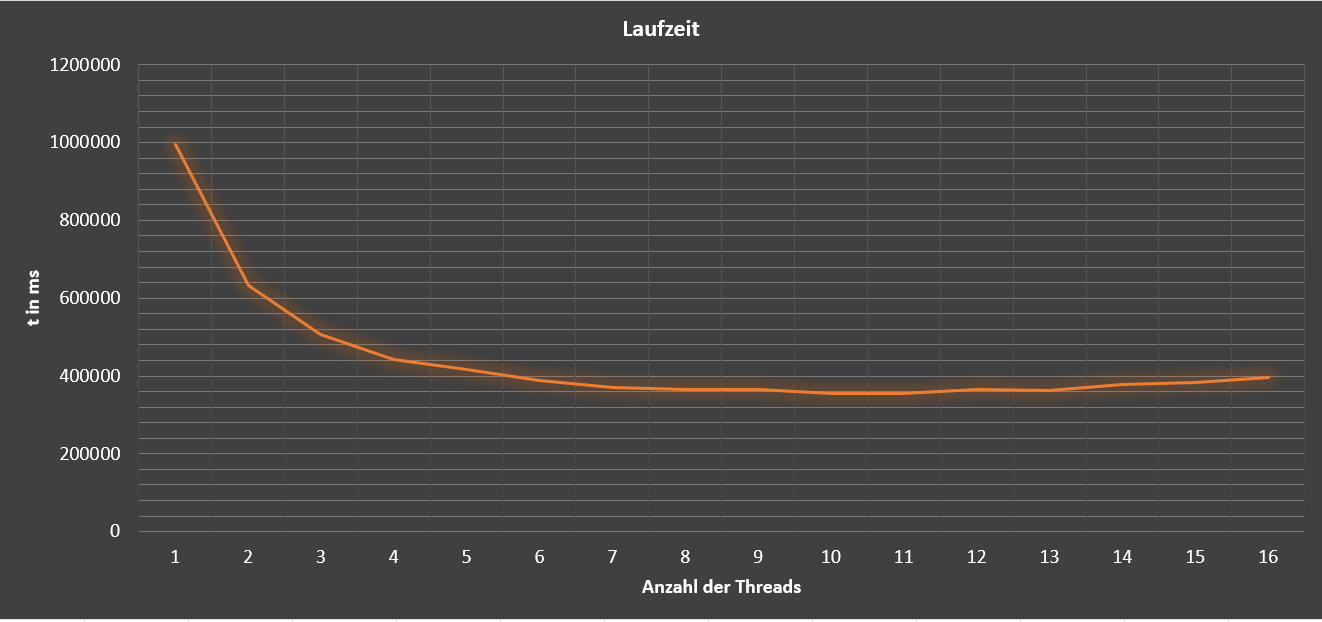
\includegraphics[width=0.8\textwidth]{Base64LaufzeitPic}
	\caption{Laufzeitdiagramm (eigene Abbildung)}
	\label{fig:Base64LaufzeitPic} 
	\end{center}
\end{figure}


% !TeX root = ../my-thesis.tex
% Table generated by Excel2LaTeX from sheet 'Tabelle1'
\begin{table}[htbp]
  \centering
  \caption{durchschnittliche Leistungsaufnahme in Abh\"angigkeit von der Thread Anzahl}
    \begin{tabular}{rrrr}
    \toprule
    \multicolumn{1}{c}{Threads} & \multicolumn{1}{c}{\O U in mV} & \multicolumn{1}{c}{\O I in mA} & \multicolumn{1}{c}{\O P in W} \\
    \midrule
    1     & 4077,382 & 565,944 & 2,306 \\
    \midrule
    2     & 3997,636 & 733,983 & 2,931 \\
    \midrule
    3     & 4029,556 & 860,404 & 3,462 \\
    \midrule
    4     & 4056,719 & 859,178 & 3,479 \\
    \midrule
    5     & 4043,867 & 869,086 & 3,505 \\
    \midrule
    6     & 4028,429 & 900,618 & 3,621 \\
    \midrule
    7     & 4017,545 & 923,407 & 3,705 \\
    \midrule
    8     & 4042,727 & 933,792 & 3,772 \\
    \midrule
    9     & 4063,227 & 901,938 & 3,662 \\
    \midrule
    10    & 4046,045 & 934,489 & 3,775 \\
    \midrule
    11    & 4034,455 & 948,283 & 3,824 \\
    \midrule
    12    & 4074,458 & 856,408 & 3,485 \\
    \midrule
    13    & 4049,000 & 962,385 & 3,486 \\
    \midrule
    14    & 4063,917 & 915,918 & 3,586 \\
    \midrule
    15    & 4021,708 & 926,291 & 3,726 \\
    \midrule
    16    & 4023,542 & 946,001 & 3,806 \\
    \bottomrule
    \end{tabular}%
  \label{tab:Base64Leistung}%
\end{table}%


\begin{figure}[h]
	\begin{center}	 
	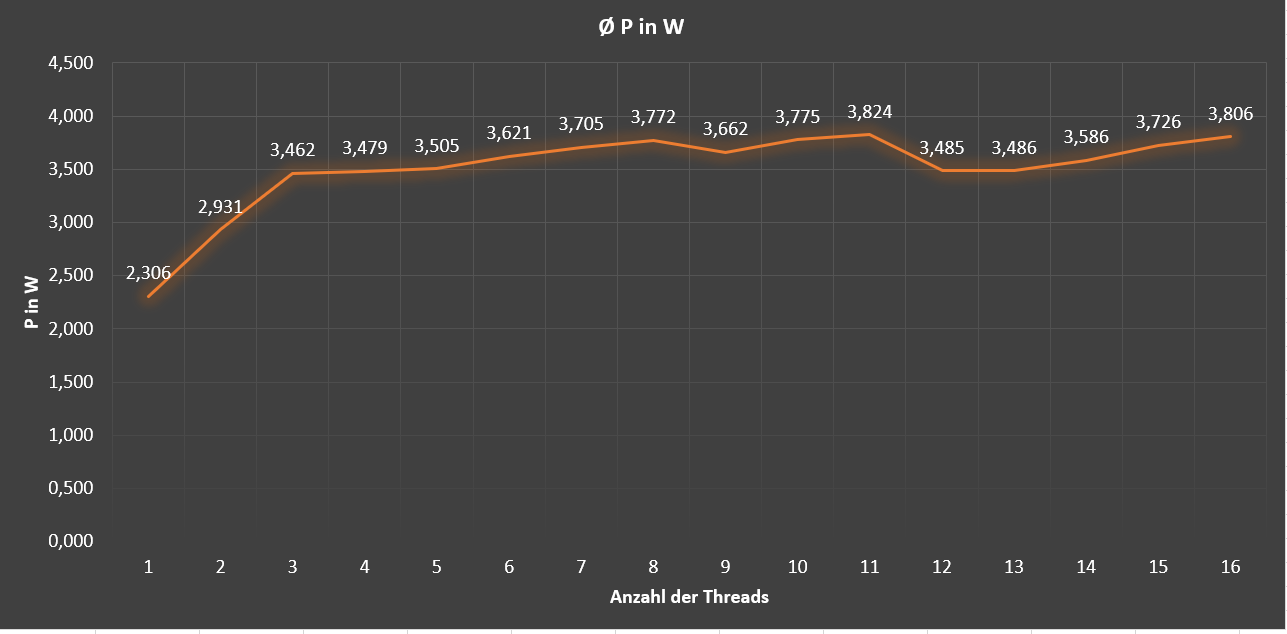
\includegraphics[width=0.8\textwidth]{Base64LeistungPic}
	\caption{durchschnittliche elektrische Leistung in Abhängigkeit von der Thread Anzahl (eigene Abbildung)}
	\label{fig:Base64LeistungPic} 
	\end{center}
\end{figure}

% !TeX root = ../my-thesis.tex
% Table generated by Excel2LaTeX from sheet 'Tabelle1'
\begin{table}[htbp]
  \centering
  \caption{elektrische Arbeit in Abhängigkeit von der Thread Anzahl}
    \begin{tabular}{rr}
    \toprule
    \multicolumn{1}{c}{Threads} & \multicolumn{1}{c}{W in Ws} \\
    \midrule
    1     & 2330,170 \\
    \midrule
    2     & 1891,658 \\
    \midrule
    3     & 1815,574 \\
    \midrule
    4     & 1594,628 \\
    \midrule
    5     & 1532,691 \\
    \midrule
    6     & 1473,056 \\
    \midrule
    7     & 1347,732 \\
    \midrule
    8     & 1296,977 \\
    \midrule
    9     & 1252,836 \\
    \midrule
    10    & 1290,069 \\
    \midrule
    11    & 1306,284 \\
    \midrule
    12    & 1316,109 \\
    \midrule
    13    & 1322,537 \\
    \midrule
    14    & 1374,502 \\
    \midrule
    15    & 1393,833 \\
    \midrule
    16    & 1409,848 \\
    \bottomrule
    \end{tabular}%
  \label{tab:Base64Arbeit}%
\end{table}%


\begin{figure}[H]
	\begin{center}	 
	\includegraphics[width=0.95\textwidth]{Base64LeistungFlächePic}
	\caption{Verlauf der elektrischen Leistung mit einem Thread (eigene Abbildung)}
	\label{fig:Base64LeistungFlächePic} 
	\end{center}
\end{figure}

\begin{figure}[H]
	\begin{center}	 
	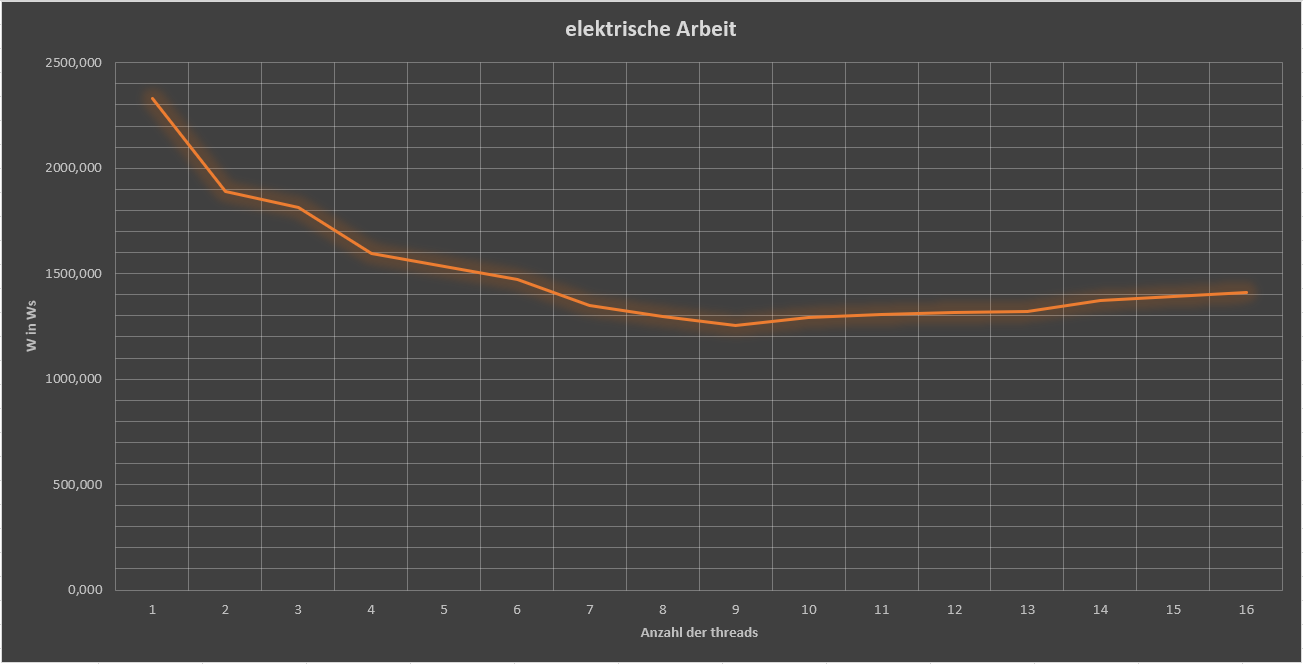
\includegraphics[width=0.95\textwidth]{Base64ArbeitPic}
	\caption{elektrische Arbeit in Abhängigkeit der Thread Anzahl(eigene Abbildung)}
	\label{fig:Base64ArbeitPic} 
	\end{center}
\end{figure}


\section{Auswertung}
% !TeX root = ../my-thesis.tex
\chapter{Rekursive und Iterative Verfahren im Vergleich}
\section{Rekursion und Iteration Vorbetrachtung}
\section{Gegenüberstellung anhand verschiedener Merge Sort Varianten}
\subsection{Rekursiver Merge Sort}
\subsection{Iterativer Merge Sort}
\subsection{Paralleler Merge Sort}
\section{Auswertung der Messung}

% Table generated by Excel2LaTeX from sheet 'Tabelle1'
\begin{table}[htbp]
  \centering
  \caption{durchschnittliche elektrische Leistung, Stromst\"arke, Spannung der Merge Sort Verfahren}
    \begin{tabular}{lrrr}
    \toprule
    Merge Sort Variante & \multicolumn{1}{l}{\O U in mV} & \multicolumn{1}{l}{\O I in mA} & \multicolumn{1}{l}{\O P in Watt} \\
    \midrule
    rekursiv & 4115,286 & 495,052 & 2,037 \\
    \midrule
    iterativ & 4148,460 & 487,577 & 2,022 \\
    \midrule
    parallel & 4111,500 & 778,158 & 3,197 \\
    \bottomrule
    \end{tabular}%
  \label{tab:MergeSortLeistung}%
\end{table}%


\begin{figure}[H]
	\begin{center}	 
	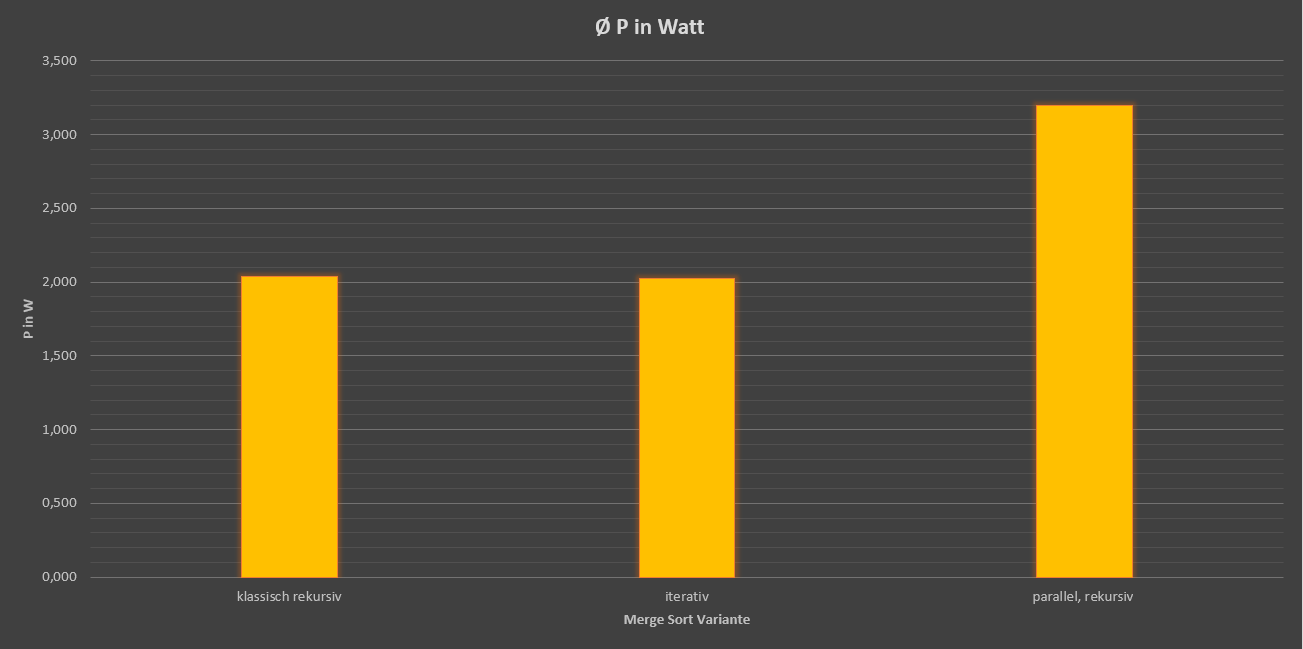
\includegraphics[width=0.8\textwidth]{MergeSortLeistungPic}
	\caption{Merge Sort: durchschnittliche elektrische Leistung pro Verfahren (eigene Abbildung)}
	\label{fig:MergeSortLeistungPic} 
	\end{center}
\end{figure}

% Table generated by Excel2LaTeX from sheet 'Tabelle1'
\begin{table}[htbp]
  \centering
  \caption{elektrische Arbeit und Laufzeit der Merge Sort Varianten Gegen\"uberstellung}
    \begin{tabular}{lrr}
    \toprule
    Merge Sort Variante & \multicolumn{1}{l}{t in s} & \multicolumn{1}{l}{W in Ws} \\
    \midrule
    rekursiv & 804,252 & 1662,462 \\
    \midrule
    iterativ & 714,388 & 1471,137 \\
    \midrule
    parallel & 284,021 & 979,787 \\
    \bottomrule
    \end{tabular}%
  \label{tab:MergeSortLaufzeitArbeit}%
\end{table}%


\begin{figure}[H]
	\begin{center}	 
	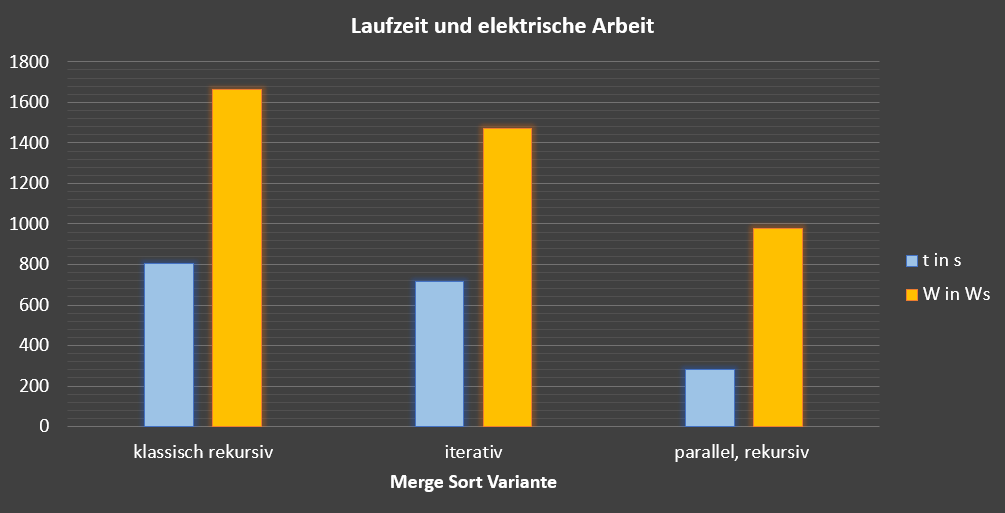
\includegraphics[width=0.8\textwidth]{MergeSortLaufzeitArbeitPic}
	\caption{Merge Sort: Gegenüberstellung von Laufzeiten und elektrischer Arbeit (eigene Abbildung)}
	\label{fig:MergeSortLaufzeitArbeitPic} 
	\end{center}
\end{figure}

\include{Content/Auswertung}

\cleardoublepage

\printbibliography % Print the bibliography
\cleardoublepage

\makedeclarationofauthorship % print the declaration of authorship

\appendix % Begin the appendix. Chapters begin with letters
\pagenumbering{Roman} %page numbers as capital roman numbers
\setcounter{page}{1} % restart page numbers from one
% !TeX root = ../my-thesis.tex
\chapter{\appendixname}\label{sec:appendix}

\section{Messwerte der parallelen Base64-Kodierung}

% !TeX root = ../my-thesis.tex
% Table generated by Excel2LaTeX from sheet 'Tabelle1'
\begin{longtable}[c]{ccccc}
\caption{Base64-Kodierung mit einem Threads} \\
\label{tab:Base64MessungThreadEins}\\
\hline
{$\Delta$ t in s} & {P in Watt} & {I in mA} & {U in mV} & {$\Delta$ W in Ws} \\
\hline
\endfirsthead
\hline
$\Delta$ t in s & P in Watt & I in mA & U in mV & $\Delta$ W in Ws \\
\hline
\endhead
\hline
\endfoot
\hline
 \midrule
    0     & 0,498474675 & 119,61 & 4167,5 & \multicolumn{1}{r}{51,625943} \\
    \midrule
    30    & 2,94325486 & 717,08 & 4104,5 & \multicolumn{1}{r}{73,585476} \\
    \midrule
    60    & 1,96244354 & 478,12 & 4104,5 & \multicolumn{1}{r}{73,576857} \\
    \midrule
    90    & 2,94268023 & 716,94 & 4104,5 & \multicolumn{1}{r}{73,419077} \\
    \midrule
    120   & 1,9519249 & 478,12 & 4082,5 & \multicolumn{1}{r}{73,20147} \\
    \midrule
    150   & 2,928173125 & 717,25 & 4082,5 & \multicolumn{1}{r}{73,200246} \\
    \midrule
    180   & 1,95184325 & 478,1 & 4082,5 & \multicolumn{1}{r}{51,231905} \\
    \midrule
    210   & 1,463617075 & 358,51 & 4082,5 & \multicolumn{1}{r}{65,863993} \\
    \midrule
    240   & 2,9273158 & 717,04 & 4082,5 & \multicolumn{1}{r}{73,182487} \\
    \midrule
    270   & 1,95151665 & 478,02 & 4082,5 & \multicolumn{1}{r}{73,194122} \\
    \midrule
    300   & 2,928091475 & 717,23 & 4082,5 & \multicolumn{1}{r}{73,199021} \\
    \midrule
    330   & 1,95184325 & 478,1 & 4082,5 & \multicolumn{1}{r}{73,1782} \\
    \midrule
    360   & 2,926703425 & 716,89 & 4082,5 & \multicolumn{1}{r}{73,1782} \\
    \midrule
    390   & 1,95184325 & 478,1 & 4082,5 & \multicolumn{1}{r}{51,236804} \\
    \midrule
    420   & 1,463943675 & 358,59 & 4082,5 & \multicolumn{1}{r}{65,618469} \\
    \midrule
    450   & 2,910620905 & 716,99 & 4059,5 & \multicolumn{1}{r}{72,766538} \\
    \midrule
    480   & 1,940481595 & 478,01 & 4059,5 & \multicolumn{1}{r}{72,773845} \\
    \midrule
    510   & 2,911108045 & 717,11 & 4059,5 & \multicolumn{1}{r}{72,775671} \\
    \midrule
    540   & 1,94060338 & 478,04 & 4059,5 & \multicolumn{1}{r}{101,86706} \\
    \midrule
    570   & 4,85053417 & 1194,86 & 4059,5 & \multicolumn{1}{r}{94,594063} \\
    \midrule
    600   & 1,4557367 & 358,6 & 4059,5 & \multicolumn{1}{r}{65,493537} \\
    \midrule
    630   & 2,91049912 & 716,96 & 4059,5 & \multicolumn{1}{r}{72,763493} \\
    \midrule
    660   & 1,940400405 & 477,99 & 4059,5 & \multicolumn{1}{r}{72,779934} \\
    \midrule
    690   & 2,911595185 & 717,23 & 4059,5 & \multicolumn{1}{r}{72,784196} \\
    \midrule
    720   & 1,94068457 & 478,06 & 4059,5 & \multicolumn{1}{r}{50,938403} \\
    \midrule
    750   & 1,455208965 & 358,47 & 4059,5 & \multicolumn{1}{r}{72,780543} \\
    \midrule
    780   & 3,39682722 & 836,76 & 4059,5 & \multicolumn{1}{r}{72,781152} \\
    \midrule
    810   & 1,45524956 & 358,48 & 4059,5 & \multicolumn{1}{r}{65,509978} \\
    \midrule
    840   & 2,912082325 & 717,35 & 4059,5 & \multicolumn{1}{r}{72,783587} \\
    \midrule
    870   & 1,940156835 & 477,93 & 4059,5 & \multicolumn{1}{r}{73,074451} \\
    \midrule
    900   & 2,93147325 & 717,18 & 4087,5 & \multicolumn{1}{r}{73,284992} \\
    \midrule
    930   & 1,954192875 & 478,09 & 4087,5 & \multicolumn{1}{r}{73,293576} \\
    \midrule
    960   & 2,9320455 & 717,32 & 4087,5 & \multicolumn{1}{r}{58,633144} \\
    \midrule
    990   & 0,97683075 & 238,98 & 4087,5 &  \\
\end{longtable}



% Table generated by Excel2LaTeX from sheet 'Tabelle1'

\begin{longtable}[c]{ccccc}
\caption{Base64-Kodierung mit zwei Threads} \\
\label{tab:Base64MessungThreadZwei}\\
\hline
{$\Delta$ t in s} & {P in Watt} & {I in mA} & {U in mV} & {$\Delta$ W in Ws} \\
\hline
\endfirsthead
\hline
$\Delta$ t in s & P in Watt & I in mA & U in mV & $\Delta$ W in Ws \\
\hline
\endhead
\hline
\endfoot
\hline
        \midrule
    0     & 1,4542958 & 358,51 & 4056,5 & 71,62824 \\
    \midrule
    30    & 3,3209202 & 836,82 & 3968,5 & 120,9694 \\
    \midrule
    60    & 4,7437068 & 1195,34 & 3968,5 & 113,92106 \\
    \midrule
    90    & 2,8510306 & 717,06 & 3976  & 92,665054 \\
    \midrule
    120   & 3,3266397 & 836,68 & 3976  & 92,708077 \\
    \midrule
    150   & 2,8538988 & 717,06 & 3980  & 142,70807 \\
    \midrule
    180   & 6,6599728 & 1673,36 & 3980  & 142,68416 \\
    \midrule
    210   & 2,8523044 & 717,2 & 3977  & 92,705063 \\
    \midrule
    240   & 3,3280331 & 836,82 & 3977  & 92,699694 \\
    \midrule
    270   & 2,8519465 & 717,11 & 3977  & 92,680008 \\
    \midrule
    300   & 3,3267207 & 836,49 & 3977  & 71,428169 \\
    \midrule
    330   & 1,4351572 & 358,61 & 4002  & 71,775555 \\
    \midrule
    360   & 3,3498798 & 836,32 & 4005,5 & 71,79318 \\
    \midrule
    390   & 1,4363322 & 358,59 & 4005,5 & 50,274633 \\
    \midrule
    420   & 1,9153099 & 478,17 & 4005,5 & 50,270427 \\
    \midrule
    450   & 1,4360519 & 358,52 & 4005,5 & 64,642161 \\
    \midrule
    480   & 2,8734255 & 717,37 & 4005,5 & 93,567547 \\
    \midrule
    510   & 3,3644109 & 836,71 & 4021  & 100,93534 \\
    \midrule
    540   & 3,364612 & 836,76 & 4021  & 95,15596 \\
    \midrule
    570   & 2,9791187 & 740,89 & 4021  & 95,07936 \\
    \midrule
    600   & 3,3595053 & 835,49 & 4021  & 71,367121 \\
    \midrule
    630   & 1,3983028 & 347,75 & 4021  &  \\
\end{longtable}
% Table generated by Excel2LaTeX from sheet 'Tabelle1'
\begin{longtable}[c]{ccccc}
\caption{Base64-Kodierung mit drei Threads} \\
\label{tab:Base64MessungThreadDrei}\\
\hline
{$\Delta$ t in s} & {P in Watt} & {I in mA} & {U in mV} & {$\Delta$ W in Ws} \\
\hline
\endfirsthead
\hline
$\Delta$ t in s & P in Watt & I in mA & U in mV & $\Delta$ W in Ws \\
\hline
\endhead
\hline
\endfoot
\hline
 \midrule
   \midrule
    0     & 1,6419644 & 398,39 & 4121,5 & 75,060991 \\
    \midrule
    30    & 3,3621017 & 836,76 & 4018  & 115,25385 \\
    \midrule
    60    & 4,3214886 & 1075,8 & 4017  & 115,16531 \\
    \midrule
    90    & 3,3561985 & 836,54 & 4012  & 124,61148 \\
    \midrule
    120   & 4,9512337 & 1232,57 & 4017  & 123,26727 \\
    \midrule
    150   & 3,2665842 & 813,19 & 4017  & 93,312701 \\
    \midrule
    180   & 2,9542625 & 735,44 & 4017  & 114,61164 \\
    \midrule
    210   & 4,6865134 & 1166,67 & 4017  & 143,86168 \\
    \midrule
    240   & 4,9042651 & 1221,79 & 4014  & 122,87777 \\
    \midrule
    270   & 3,2875864 & 819,03 & 4014  & 114,09434 \\
    \midrule
    300   & 4,3187027 & 1075,91 & 4014  & 115,01304 \\
    \midrule
    330   & 3,3488336 & 836,79 & 4002  & 101,28922 \\
    \midrule
    360   & 3,403781 & 850,52 & 4002  & 93,422288 \\
    \midrule
    390   & 2,8243715 & 705,74 & 4002  & 93,875879 \\
    \midrule
    420   & 3,4340204 & 848,43 & 4047,5 & 103,02061 \\
    \midrule
    450   & 3,4340204 & 848,43 & 4047,5 & 94,463186 \\
    \midrule
    480   & 2,8635253 & 707,48 & 4047,5 & 72,372799 \\
    \midrule
    510   & 1,961328 & 477,79 & 4105  &  \\
\end{longtable}

% Table generated by Excel2LaTeX from sheet 'Tabelle1'

\begin{longtable}[c]{ccccc}
\caption{Base64-Kodierung mit vier Threads} \\
\label{tab:Base64MessungThreadVier}\\
\hline
{$\Delta$ t in s} & {P in Watt} & {I in mA} & {U in mV} & {$\Delta$ W in Ws} \\
\hline
\endfirsthead
\hline
$\Delta$ t in s & P in Watt & I in mA & U in mV & $\Delta$ W in Ws \\
\hline
\endhead
\hline
\endfoot
\hline
        \midrule
    0     & 3,5440048 & 838,52 & 4226,5 & 96,918029 \\
    \midrule
    30    & 2,9171972 & 716,58 & 4071  & 116,00246 \\
    \midrule
    60    & 4,8163002 & 1195,26 & 4029,5 & 144,48659 \\
    \midrule
    90    & 4,816139 & 1195,22 & 4029,5 & 122,81312 \\
    \midrule
    120   & 3,3714021 & 836,68 & 4029,5 & 144,50109 \\
    \midrule
    150   & 6,2620042 & 1554,04 & 4029,5 & 144,50472 \\
    \midrule
    180   & 3,3716438 & 836,74 & 4029,5 & 93,842127 \\
    \midrule
    210   & 2,884498 & 717,18 & 4022  & 115,37268 \\
    \midrule
    240   & 4,807014 & 1195,18 & 4022  & 122,38665 \\
    \midrule
    270   & 3,3520959 & 836,56 & 4007  & 93,709133 \\
    \midrule
    300   & 2,8951796 & 717,25 & 4036,5 & 94,09021 \\
    \midrule
    330   & 3,377501 & 836,74 & 4036,5 & 94,075678 \\
    \midrule
    360   & 2,8942109 & 717,01 & 4036,5 & 94,444106 \\
    \midrule
    390   & 3,4020629 & 836,71 & 4066  & 73,181047 \\
    \midrule
    420   & 1,4766736 & 358,59 & 4118  & 44,300209 \\
    \midrule
    450   & 1,4766736 & 358,59 & 4118  &  \\
\end{longtable}


\input{Content/Anhang/Base64MessungThreadFünf}
% Table generated by Excel2LaTeX from sheet 'Tabelle1'
\begin{longtable}[c]{ccccc}
\caption{Base64-Kodierung mit sechs Threads} \\
\label{tab:Base64MessungThreadSechs}\\
\hline
{$\Delta$ t in s} & {P in Watt} & {I in mA} & {U in mV} & {$\Delta$ W in Ws} \\
\hline
\endfirsthead
\hline
$\Delta$ t in s & P in Watt & I in mA & U in mV & $\Delta$ W in Ws \\
\hline
\endhead
\hline
\endfoot
\hline
       \midrule
    0     & 1,7253043 & 418,56 & 4122  & 97,568271 \\
    \midrule
    30    & 4,7792471 & 1195,26 & 3998,5 & 143,36351 \\
    \midrule
    60    & 4,77832 & 1194,58 & 4000  & 114,7068 \\
    \midrule
    90    & 2,8688 & 717,2 & 4000  & 114,81146 \\
    \midrule
    120   & 4,7852974 & 1194,98 & 4004,5 & 121,9241 \\
    \midrule
    150   & 3,3429761 & 836,79 & 3995  & 122,32258 \\
    \midrule
    180   & 4,8118623 & 1194,9 & 4027  & 115,50342 \\
    \midrule
    210   & 2,8883658 & 717,25 & 4027  & 115,53242 \\
    \midrule
    240   & 4,8137953 & 1195,38 & 4027  & 122,73511 \\
    \midrule
    270   & 3,3685452 & 836,49 & 4027  & 122,74992 \\
    \midrule
    300   & 4,8147826 & 1195,18 & 4028,5 & 115,5323 \\
    \midrule
    330   & 2,8873704 & 717,27 & 4025,5 & 93,81146 \\
    \midrule
    360   & 3,3667269 & 836,35 & 4025,5 & 72,495113 \\
    \midrule
    390   & 1,4662806 & 358,46 & 4090,5 &  \\
\end{longtable}



% Table generated by Excel2LaTeX from sheet 'Tabelle1'

\begin{longtable}[c]{ccccc}
\caption{Base64-Kodierung mit sieben Threads} \\
\label{tab:Base64MessungThreadSieben}\\
\hline
{$\Delta$ t in s} & {P in Watt} & {I in mA} & {U in mV} & {$\Delta$ W in Ws} \\
\hline
\endfirsthead
\hline
$\Delta$ t in s & P in Watt & I in mA & U in mV & $\Delta$ W in Ws \\
\hline
\endhead
\hline
\endfoot
\hline
    \midrule
    0     & 3,4421244 & 834,05 & 4127  & \multicolumn{1}{r}{116,60426} \\
    \midrule
    30    & 4,3314929 & 1075,88 & 4026  & \multicolumn{1}{r}{137,10644} \\
    \midrule
    60    & 4,8089362 & 1194,47 & 4026  & \multicolumn{1}{r}{122,52145} \\
    \midrule
    90    & 3,3591606 & 835,82 & 4019  & \multicolumn{1}{r}{121,45647} \\
    \midrule
    120   & 4,7379371 & 1194,94 & 3965  & \multicolumn{1}{r}{113,87274} \\
    \midrule
    150   & 2,8535791 & 717,25 & 3978,5 & \multicolumn{1}{r}{114,67824} \\
    \midrule
    180   & 4,791637 & 1195,22 & 4009  & \multicolumn{1}{r}{122,19191} \\
    \midrule
    210   & 3,3544907 & 836,74 & 4009  & \multicolumn{1}{r}{122,19432} \\
    \midrule
    240   & 4,7917973 & 1195,26 & 4009  & \multicolumn{1}{r}{115,00037} \\
    \midrule
    270   & 2,874894 & 717,11 & 4009  & \multicolumn{1}{r}{93,852742} \\
    \midrule
    300   & 3,3819555 & 836,6 & 4042,5 & \multicolumn{1}{r}{72,758018} \\
    \midrule
    330   & 1,468579 & 358,19 & 4100  & \multicolumn{1}{r}{95,495355} \\
    \midrule
    360   & 4,897778 & 1194,58 & 4100  &  \\
\end{longtable}

% !TeX root = ../my-thesis.tex
% Table generated by Excel2LaTeX from sheet 'Tabelle1'

\begin{longtable}[c]{ccccc}
\caption{Base64-Kodierung mit acht Threads} \\
\label{tab:Base64MessungThreadAcht}\\
\hline
{$\Delta$ t in s} & {P in Watt} & {I in mA} & {U in mV} & {$\Delta$ W in Ws} \\
\hline
\endfirsthead
\hline
$\Delta$ t in s & P in Watt & I in mA & U in mV & $\Delta$ W in Ws \\
\hline
\endhead
\hline
\endfoot
\hline
 \midrule
    0     & 1,9986448 & 478,66 & 4175,5 & 102,08178 \\
    \midrule
    30    & 4,8068071 & 1194,98 & 4022,5 & 143,86909 \\
    \midrule
    60    & 4,7844657 & 1195,22 & 4003  & 115,29143 \\
    \midrule
    90    & 2,9016294 & 717,16 & 4046  & 115,92449 \\
    \midrule
    120   & 4,8266698 & 1195,46 & 4037,5 & 123,85654 \\
    \midrule
    150   & 3,4304327 & 853,66 & 4018,5 & 122,11257 \\
    \midrule
    180   & 4,7104053 & 1172,18 & 4018,5 & 114,48111 \\
    \midrule
    210   & 2,9216687 & 725,61 & 4026,5 & 93,773159 \\
    \midrule
    240   & 3,3298752 & 826,99 & 4026,5 & 93,406207 \\
    \midrule
    270   & 2,8972052 & 717,13 & 4040  & 95,228804 \\
    \midrule
    300   & 3,4513818 & 838,63 & 4115,5 & 103,29823 \\
    \midrule
    330   & 3,4351667 & 834,69 & 4115,5 & 73,653663 \\
    \midrule
    360   & 1,4750775 & 358,42 & 4115,5 &  \\
\end{longtable}
% Table generated by Excel2LaTeX from sheet 'Tabelle1'

\begin{longtable}[c]{ccccc}
\caption{Base64-Kodierung mit neun Threads} \\
\label{tab:Base64MessungThreadNeun}\\
\hline
{$\Delta$ t in s} & {P in Watt} & {I in mA} & {U in mV} & {$\Delta$ W in Ws} \\
\hline
\endfirsthead
\hline
$\Delta$ t in s & P in Watt & I in mA & U in mV & $\Delta$ W in Ws \\
\hline
\endhead
\hline
\endfoot
\hline
    \midrule
    0     & 1,49514709 & 359,54 & 4158,5 & 95,144258 \\
    \midrule
    30    & 4,84780347 & 1195,66 & 4054,5 & 123,60001 \\
    \midrule
    60    & 3,392197425 & 836,65 & 4054,5 & 123,58132 \\
    \midrule
    90    & 4,846557 & 1195,5 & 4054  & 116,27285 \\
    \midrule
    120   & 2,904966015 & 717,01 & 4051,5 & 115,42281 \\
    \midrule
    150   & 4,78988766 & 1195,38 & 4007  & 122,07634 \\
    \midrule
    180   & 3,34853523 & 836,82 & 4001,5 & 94,27973 \\
    \midrule
    210   & 2,936780125 & 717,25 & 4094,5 & 117,45913 \\
    \midrule
    240   & 4,89382829 & 1195,22 & 4094,5 & 124,7979 \\
    \midrule
    270   & 3,42603193 & 836,74 & 4094,5 & 73,413566 \\
    \midrule
    300   & 1,46820581 & 358,58 & 4094,5 & 73,39944 \\
    \midrule
    330   & 3,425090195 & 836,51 & 4094,5 & 73,388385 \\
    \midrule
    360   & 1,4674688 & 358,4 & 4094,5 &  \\
\end{longtable}


% Table generated by Excel2LaTeX from sheet 'Tabelle1'

\begin{longtable}[c]{ccccc}
\caption{Base64-Kodierung mit zehn Threads} \\
\label{tab:Base64MessungThreadZehn}\\
\hline
{$\Delta$ t in s} & {P in Watt} & {I in mA} & {U in mV} & {$\Delta$ W in Ws} \\
\hline
\endfirsthead
\hline
$\Delta$ t in s & P in Watt & I in mA & U in mV & $\Delta$ W in Ws \\
\hline
\endhead
\hline
\endfoot
\hline
    \midrule
    0     & 1,4831672 & 358,99 & 4131,5 & 94,356503 \\
    \midrule
    30    & 4,8072663 & 1195,54 & 4021  & 144,2011 \\
    \midrule
    60    & 4,8061405 & 1195,26 & 4021  & 122,49566 \\
    \midrule
    90    & 3,360237 & 836,4 & 4017,5 & 122,33737 \\
    \midrule
    120   & 4,7955878 & 1195,46 & 4011,5 & 143,70801 \\
    \midrule
    150   & 4,784946 & 1195,34 & 4003  & 115,36205 \\
    \midrule
    180   & 2,9058573 & 717,23 & 4051,5 & 116,48756 \\
    \midrule
    210   & 4,85998 & 1195,42 & 4065,5 & 123,91217 \\
    \midrule
    240   & 3,4008314 & 836,51 & 4065,5 & 94,889712 \\
    \midrule
    270   & 2,9251494 & 717,3 & 4078  & 95,145713 \\
    \midrule
    300   & 3,4178981 & 836,49 & 4086  & 73,236647 \\
    \midrule
    330   & 1,464545 & 358,43 & 4086  & 43,936349 \\
    \midrule
    360   & 1,464545 & 358,43 & 4086  &  \\
\end{longtable}
% !TeX root = ../my-thesis.tex
% Table generated by Excel2LaTeX from sheet 'Tabelle1'

\begin{longtable}[c]{ccccc}
\caption{Base64-Kodierung mit 11 Threads} \\
\label{tab:Base64MessungThreadElf}\\
\hline
{$\Delta$ t in s} & {P in Watt} & {I in mA} & {U in mV} & {$\Delta$ W in Ws} \\
\hline
\endfirsthead
\hline
$\Delta$ t in s & P in Watt & I in mA & U in mV & $\Delta$ W in Ws \\
\hline
\endhead
\hline
\endfoot
\hline
     \midrule
    0     & 1,4939819 & 358,57 & 4166,5 & 53,453075 \\
    \midrule
    30    & 2,0695564 & 511,57 & 4045,5 & 81,261329 \\
    \midrule
    60    & 3,3478655 & 835,4 & 4007,5 & 122,07526 \\
    \midrule
    90    & 4,7904854 & 1195,38 & 4007,5 & 122,13338 \\
    \midrule
    120   & 3,3517401 & 836,68 & 4006  & 114,94202 \\
    \midrule
    150   & 4,3110616 & 1075,48 & 4008,5 & 115,51974 \\
    \midrule
    180   & 3,3902547 & 836,79 & 4051,5 & 144,88576 \\
    \midrule
    210   & 6,2687957 & 1553,99 & 4034  & 144,67154 \\
    \midrule
    240   & 3,3759739 & 836,88 & 4034  & 122,97205 \\
    \midrule
    270   & 4,8221629 & 1195,38 & 4034  & 115,94416 \\
    \midrule
    300   & 2,9074477 & 717,18 & 4054  & 95,005176 \\
    \midrule
    330   & 3,4262307 & 836,38 & 4096,5 & 73,420545 \\
    \midrule
    360   & 1,4684724 & 358,47 & 4096,5 &  \\
\end{longtable}
\input{Content/Anhang/Base64MessungThreadZwölf}
% Table generated by Excel2LaTeX from sheet 'Tabelle1'
\begin{longtable}[c]{ccccc}
\caption{Base64-Kodierung mit 13 Threads} \\
\label{tab:Base64MessungThreadDreizehn}\\
\hline
{$\Delta$ t in s} & {P in Watt} & {I in mA} & {U in mV} & {$\Delta$ W in Ws} \\
\hline
\endfirsthead
\hline
$\Delta$ t in s & P in Watt & I in mA & U in mV & $\Delta$ W in Ws \\
\hline
\endhead
\hline
\endfoot
\hline
 \midrule
    0     & 1,9986448 & 478,66 & 4175,5 & 102,08178 \\
    \midrule
    30    & 4,8068071 & 1194,98 & 4022,5 & 143,86909 \\
    \midrule
    60    & 4,7844657 & 1195,22 & 4003  & 115,29143 \\
    \midrule
    90    & 2,9016294 & 717,16 & 4046  & 115,92449 \\
    \midrule
    120   & 4,8266698 & 1195,46 & 4037,5 & 123,85654 \\
    \midrule
    150   & 3,4304327 & 853,66 & 4018,5 & 122,11257 \\
    \midrule
    180   & 4,7104053 & 1172,18 & 4018,5 & 114,48111 \\
    \midrule
    210   & 2,9216687 & 725,61 & 4026,5 & 93,773159 \\
    \midrule
    240   & 3,3298752 & 826,99 & 4026,5 & 93,406207 \\
    \midrule
    270   & 2,8972052 & 717,13 & 4040  & 95,228804 \\
    \midrule
    300   & 3,4513818 & 838,63 & 4115,5 & 103,29823 \\
    \midrule
    330   & 3,4351667 & 834,69 & 4115,5 & 73,653663 \\
    \midrule
    360   & 1,4750775 & 358,42 & 4115,5 &  \\
\end{longtable}
% Table generated by Excel2LaTeX from sheet 'Tabelle1'

\begin{longtable}[c]{ccccc}
\caption{Base64-Kodierung mit 14 Threads} \\
\label{tab:Base64MessungThreadVierzehn}\\
\hline
{$\Delta$ t in s} & {P in Watt} & {I in mA} & {U in mV} & {$\Delta$ W in Ws} \\
\hline
\endfirsthead
\hline
$\Delta$ t in s & P in Watt & I in mA & U in mV & $\Delta$ W in Ws \\
\hline
\endhead
\hline
\endfoot
\hline
           \midrule
    0     & 0,3662014 & 88,54 & 4136  & 49,107698 \\
    \midrule
    30    & 2,9076451 & 716,61 & 4057,5 & 116,14957 \\
    \midrule
    60    & 4,8356598 & 1194,58 & 4048  & 123,57061 \\
    \midrule
    90    & 3,4023806 & 835,35 & 4073  & 124,61591 \\
    \midrule
    120   & 4,905347 & 1195,26 & 4104  & 117,25119 \\
    \midrule
    150   & 2,9113989 & 717,27 & 4059  & 145,34967 \\
    \midrule
    180   & 6,7785788 & 1673,31 & 4051  & 145,57678 \\
    \midrule
    210   & 2,9265401 & 716,85 & 4082,5 & 94,606792 \\
    \midrule
    240   & 3,3805794 & 836,57 & 4041  & 93,689882 \\
    \midrule
    270   & 2,8654128 & 717,16 & 3995,5 & 115,22815 \\
    \midrule
    300   & 4,816464 & 1193,08 & 4037  & 101,55225 \\
    \midrule
    330   & 1,9536861 & 478,2 & 4085,5 & 73,741448 \\
    \midrule
    360   & 2,9624104 & 716,77 & 4133  & 74,061707 \\
    \midrule
    390   & 1,9750367 & 477,87 & 4133  &  \\
\end{longtable}



\input{Content/Anhang/Base64MessungThreadFünfzehn}
% Table generated by Excel2LaTeX from sheet 'Tabelle1'

\begin{longtable}[c]{ccccc}
\caption{Base64-Kodierung mit 16 Threads} \\
\label{tab:Base64MessungThreadSechszehn}\\
\hline
{$\Delta$ t in s} & {P in Watt} & {I in mA} & {U in mV} & {$\Delta$ W in Ws} \\
\hline
\endfirsthead
\hline
$\Delta$ t in s & P in Watt & I in mA & U in mV & $\Delta$ W in Ws \\
\hline
\endhead
\hline
\endfoot
\hline
           \midrule
    0     & 0,6952572 & 167,29 & 4156  & 53,901095 \\
    \midrule
    30    & 2,8981491 & 716,92 & 4042,5 & 115,38239 \\
    \midrule
    60    & 4,7940101 & 1194,62 & 4013  & 122,27109 \\
    \midrule
    90    & 3,3573962 & 836,63 & 4013  & 122,26869 \\
    \midrule
    120   & 4,7938495 & 1194,58 & 4013  & 115,08261 \\
    \midrule
    150   & 2,8783243 & 717,25 & 4013  & 115,25181 \\
    \midrule
    180   & 4,8051295 & 1194,86 & 4021,5 & 122,53776 \\
    \midrule
    210   & 3,3640548 & 835,79 & 4025  & 122,62706 \\
    \midrule
    240   & 4,8110825 & 1195,3 & 4025  & 115,45407 \\
    \midrule
    270   & 2,8858554 & 717,25 & 4023,5 & 115,54713 \\
    \midrule
    300   & 4,8172869 & 1195,06 & 4031  & 122,86125 \\
    \midrule
    330   & 3,3734633 & 836,88 & 4031  & 93,947494 \\
    \midrule
    360   & 2,889703 & 716,87 & 4031  & 72,715504 \\
    \midrule
    390   & 1,9579973 & 477,91 & 4097  &  \\
\end{longtable}


\section{Messwerte der Mergesort-Implementierungen}

% Table generated by Excel2LaTeX from sheet 'Tabelle1'

\begin{longtable}[c]{ccccc}
\caption{rekursiver Mergesort} \\
\label{tab:MergeSortMessungRekursive}\\
\hline
{$\Delta$ t in s} & {P in Watt} & {I in mA} & {U in mV} & {$\Delta$ W in Ws} \\
\hline
\endfirsthead
\hline
$\Delta$ t in s & P in Watt & I in mA & U in mV & $\Delta$ W in Ws \\
\hline
\endhead
\hline
\endfoot
\hline
      \midrule
    0     & 1,74560854 & 418,21 & 4174  & 52,340027 \\
    \midrule
    30    & 1,7437266 & 418,21 & 4169,5 & 48,3180287 \\
    \midrule
    60    & 1,47747532 & 358,48 & 4121,5 & 51,7176124 \\
    \midrule
    90    & 1,97036551 & 478,07 & 4121,5 & 73,8754146 \\
    \midrule
    120   & 2,95466214 & 716,89 & 4121,5 & 66,4876259 \\
    \midrule
    150   & 1,47784626 & 358,57 & 4121,5 & 51,7151395 \\
    \midrule
    180   & 1,96982971 & 477,94 & 4121,5 & 73,8809786 \\
    \midrule
    210   & 2,95556887 & 717,11 & 4121,5 & 73,8822151 \\
    \midrule
    240   & 1,96991214 & 477,96 & 4121,5 & 51,7108119 \\
    \midrule
    270   & 1,47747532 & 358,48 & 4121,5 & 44,3205503 \\
    \midrule
    300   & 1,47722803 & 358,42 & 4121,5 & 73,6576697 \\
    \midrule
    330   & 3,43328328 & 836,57 & 4104  & 73,5635844 \\
    \midrule
    360   & 1,47095568 & 358,42 & 4104  & 44,13852 \\
    \midrule
    390   & 1,47161232 & 358,58 & 4104  & 51,5004804 \\
    \midrule
    420   & 1,96175304 & 478,01 & 4104  & 73,5598908 \\
    \midrule
    450   & 2,94223968 & 716,92 & 4104  & 73,5629688 \\
    \midrule
    480   & 1,96195824 & 478,06 & 4104  & 51,4930932 \\
    \midrule
    510   & 1,47091464 & 358,41 & 4104  & 73,5592752 \\
    \midrule
    540   & 3,43303704 & 836,51 & 4104  & 73,5660468 \\
    \midrule
    570   & 1,47136608 & 358,52 & 4104  & 44,1403668 \\
    \midrule
    600   & 1,47132504 & 358,51 & 4104  & 73,5586596 \\
    \midrule
    630   & 3,4325856 & 836,4 & 4104  & 73,5586596 \\
    \midrule
    660   & 1,47132504 & 358,51 & 4104  & 44,1403668 \\
    \midrule
    690   & 1,47136608 & 358,52 & 4104  & 51,4955556 \\
    \midrule
    720   & 1,96167096 & 477,99 & 4104  & 73,5568128 \\
    \midrule
    750   & 2,94211656 & 716,89 & 4104  & 73,554966 \\
    \midrule
    780   & 1,96154784 & 477,96 & 4104  & 51,6062553 \\
    \midrule
    810   & 1,47886918 & 358,34 & 4127  &  \\
\end{longtable}

% Table generated by Excel2LaTeX from sheet 'Tabelle1'

\begin{longtable}[c]{ccccc}
\caption{iterativer Mergesort} \\
\label{tab:MergeSortMessungIterativ}\\
\hline
{$\Delta$ t in s} & {P in Watt} & {I in mA} & {U in mV} & {$\Delta$ W in Ws} \\
\hline
\endfirsthead
\hline
$\Delta$ t in s & P in Watt & I in mA & U in mV & $\Delta$ W in Ws \\
\hline
\endhead
\hline
\endfoot
\hline
  \midrule
    0     & 1,53241658 & 359,09 & 4267,5 & 52,8862313 \\
    \midrule
    30    & 1,99333218 & 477,96 & 4170,5 & 52,327472 \\
    \midrule
    60    & 1,49516596 & 358,51 & 4170,5 & 67,0483405 \\
    \midrule
    90    & 2,97472341 & 717,06 & 4148,5 & 74,3662184 \\
    \midrule
    120   & 1,98302449 & 478,01 & 4148,5 & 52,0445919 \\
    \midrule
    150   & 1,48661498 & 358,35 & 4148,5 & 44,6108948 \\
    \midrule
    180   & 1,48744468 & 358,55 & 4148,5 & 74,3487947 \\
    \midrule
    210   & 3,46914164 & 836,24 & 4148,5 & 74,3469279 \\
    \midrule
    240   & 1,48732022 & 358,52 & 4148,5 & 52,0570374 \\
    \midrule
    270   & 1,98314894 & 478,04 & 4148,5 & 74,3680853 \\
    \midrule
    300   & 2,97472341 & 717,06 & 4148,5 & 66,9300322 \\
    \midrule
    330   & 1,48727874 & 358,51 & 4148,5 & 52,0564151 \\
    \midrule
    360   & 1,98314894 & 478,04 & 4148,5 & 51,9387258 \\
    \midrule
    390   & 1,47943278 & 358,52 & 4126,5 & 73,9730833 \\
    \midrule
    420   & 3,45210611 & 836,57 & 4126,5 & 73,9699884 \\
    \midrule
    450   & 1,47922646 & 358,47 & 4126,5 & 44,3743178 \\
    \midrule
    480   & 1,4790614 & 358,43 & 4126,5 & 73,98113 \\
    \midrule
    510   & 3,45301394 & 836,79 & 4126,5 & 73,9842248 \\
    \midrule
    540   & 1,47926772 & 358,48 & 4126,5 & 44,3774126 \\
    \midrule
    570   & 1,47922646 & 358,47 & 4126,5 & 51,771069 \\
    \midrule
    600   & 1,97217815 & 477,93 & 4126,5 & 74,235791 \\
    \midrule
    630   & 2,97687459 & 717,06 & 4151,5 & 74,416883 \\
    \midrule
    660   & 1,98425094 & 477,96 & 4151,5 & 52,0859645 \\
    \midrule
    690   & 1,48814669 & 358,46 & 4151,5 & 44,636928 \\
    \midrule
    720   & 1,48764851 & 358,34 & 4151,5 &  \\
\end{longtable}

% Table generated by Excel2LaTeX from sheet 'Tabelle1'
\begin{longtable}[c]{ccccc}
\caption{paralleler Mergesort} \\
\label{tab:MergeSortMessungParallel}\\
\hline
{$\Delta$ t in s} & {P in Watt} & {I in mA} & {U in mV} & {$\Delta$ W in Ws} \\
\hline
\endfirsthead
\hline
$\Delta$ t in s & P in Watt & I in mA & U in mV & $\Delta$ W in Ws \\
\hline
\endhead
\hline
\endfoot
\hline
      \midrule
    0     & 3,53301535 & 838,3 & 4214,5 & 97,25161515 \\
    \midrule
    30    & 2,95042566 & 717,08 & 4114,5 & 95,81293905 \\
    \midrule
    60    & 3,43710361 & 836,38 & 4109,5 & 122,3209869 \\
    \midrule
    90    & 4,71762885 & 1149,94 & 4102,5 & 114,9022046 \\
    \midrule
    120   & 2,94251813 & 717,25 & 4102,5 & 95,60773688 \\
    \midrule
    150   & 3,431331 & 836,4 & 4102,5 & 102,7280178 \\
    \midrule
    180   & 3,41720352 & 836,32 & 4086  & 124,1934782 \\
    \midrule
    210   & 4,86236169 & 1194,39 & 4071  & 116,6696351 \\
    \midrule
    240   & 2,91561398 & 717,16 & 4065,5 & 65,9230428 \\
    \midrule
    270   & 1,47925554 & 358,26 & 4129  & 44,3776662 \\
    \midrule
    300   & 1,47925554 & 358,26 & 4129  &  \\
\end{longtable} % include the appendix
\end{document}
% ----------------------------------------------------